%% ****** Start of file aiptemplate.tex ****** %
%%
%%   This file is part of the files in the distribution of AIP substyles for REVTeX4.
%%   Version 4.1 of 9 October 2009.
%%
%
% This is a template for producing documents for use with 
% the REVTEX 4.1 document class and the AIP substyles.
% 
% Copy this file to another name and then work on that file.
% That way, you always have this original template file to use.

\documentclass[aip,graphicx]{revtex4-1}
%\documentclass[aip,reprint]{revtex4-1}
\usepackage{amsmath}
\usepackage[utf8]{inputenc}
\usepackage{graphicx}
\usepackage{xcolor}
\renewcommand{\thefigure}{S\arabic{figure}}
%\usepackage{siunitx}

\draft % marks overfull lines with a black rule on the right

\begin{document}

% Use the \preprint command to place your local institutional report number 
% on the title page in preprint mode.
% Multiple \preprint commands are allowed.
%\preprint{}

\title{Magnetic-field Assisted Assembly of Colloidal Ellipsoids}

% repeat the \author .. \affiliation  etc. as needed
% \email, \thanks, \homepage, \altaffiliation all apply to the current author.
% Explanatory text should go in the []'s, 
% actual e-mail address or url should go in the {}'s for \email and \homepage.
% Please use the appropriate macro for the type of information

% \affiliation command applies to all authors since the last \affiliation command. 
% The \affiliation command should follow the other information.

%\author{}

\author{Antara Pal}
\email{antara.pal@fkem1.lu.se}
\affiliation{Division of Physical Chemistry, Department of Chemistry, Lund University, Lund, Sweden}
\author{Carlo Andrea De Filippo}
\affiliation{XXX}
\author{Thiago H.Ito}
\affiliation{Division of Physical Chemistry, Department of Chemistry, Lund University, Lund, Sweden}
\author{Md. Arif Kamal}
\affiliation{Centre Interdisciplinaire de Nanoscience de Marseille (CINaM), CNRS, Aix Marseille University, Marseille, France}
\altaffiliation[Current Address: ]{Division of Physical Chemistry, Department of Chemistry, Lund University, Lund, Sweden}
\author{Andrei V. Petukhov}
\affiliation{Van't Hoff Laboratory for Physical and Colloid Chemistry, Utrecht University, The Netherlands}
\author{Cristiano De Michele}
\affiliation{Department of Physics, Universit\`{a} di Roma La Sapienza, I-00186 Roma, Italy}
\author{Peter Schurtenberger}
\email{peter.schurtenberger@fkem1.lu.se}
\affiliation{Division of Physical Chemistry, Department of Chemistry, Lund University, Lund, Sweden}


% Collaboration name, if desired (requires use of superscriptaddress option in \documentclass). 
% \noaffiliation is required (may also be used with the \author command).
%\collaboration{}
%\noaffiliation

%\date{\today}

%\pacs{}% insert suggested PACS numbers in braces on next line

\maketitle {}%\maketitle must follow title, authors, abstract and \pacs
\section{Smectic phase characterization}

\subsection{Real space structure}

\begin{figure}[]
\centering
\includegraphics [width=1\linewidth]{paperclip.png}
\caption{(a) Real space image of a classical smectic phase formed by colloidal rods and (b) expected x-ray diffraction pattern for it. (c) Real space image of \textit{oblate} smectic phase formed by ellipsoids and (d) expected diffraction x-ray diffraction pattern for it. (e) Smectic phase with layer fluctuation and (d) the corresponding change in the diffraction pattern.}
\label{paperclip}
\end{figure}

%Fig.\ref{paperclip}(a) shows the real space structure of a classical smectic phase consists of rod-like colloids where the particles are aligned along their long axes. As a result, the smectic layers are along their length. Fig.\ref{paperclip}(b) shows the corresponding Fourier space image or the expected x-ray diffraction pattern~\cite{kuijk2012phase, byelov2013situ}. Fig.\ref{paperclip}(c) represents the smectic phase formed by our ellipsoidal particles in the presence of an external field. One can observe that the particles are aligned with their short axes being parallel to the external field. The red doubled arrows show the spacings along the layers. There are also correlations between particles belong to different layers as shown by green lines which result in the formation of a diffused scattering line as shown in Fig.\ref{paperclip}(d) in green. Although from our drawing it seems that the long axes are also aligned, it is not true. In reality they can still rotate around the field as has been shown in Fig. 2. For the drawing, we have not considered all possible rotational conformations but only one; otherwise it will be extremely difficult to draw and point out the different spacings while including the all rotational conformations. Further, The layers in the smectic phase are not rigid but can fluctuate as can be seen in Fig.\ref{paperclip}(e) which elongated the smectic peak in vertical direction as shown by dark yellow in Fig.\ref{paperclip}(f). Combining all the aforementioned effects it is possible to understand the paperclip shape for the smectic phase in our study.

The real space structure of a classical smectic phase consisting of rod-like colloids is schematically shown in Fig.\ref{paperclip}(a). In this case the particles align along their long axes. As a result, the smectic layers form in a direction parallel to the length of the rods. The corresponding Fourier space image or the expected x-ray diffraction pattern of the aforementioned smectic phase is shown in Fig.\ref{paperclip}(b)~\cite{kuijk2012phase, byelov2013situ}. However, the smectic phase formed by ellipsoidal particles which in the presence of an external field align with their short axes parallel to the external field, has the appearance as shown in Fig.\ref{paperclip}(c). The double headed red arrows indicate the spacings along the smectic layers. Correlations between particles which belong to different layers (as indicated by green lines) results in the formation of a diffused scattering line as shown in Fig.\ref{paperclip}(d) in green. Although our schematic gives an impression that the long axes are also aligned, but this is not the case in general. As mentioned before the particles align with their short axes along the field direction and their long axes are free to rotate about this direction (Fig. 2). For the sake of clarity in illustration, we have chosen to highlight only one such possible conformation out the ensemble of all possible rotational conformations. Further it is important to note that the smectic layers in this case are not rigid but can fluctuate, Fig.\ref{paperclip}(e), resulting thereby in an elongation of the smectic peak in vertical direction as indicated by dark yellow in Fig.\ref{paperclip}(f).


\subsection{Static Structure factor}

A way to characterize the smectic phase obtained from the simulations is provided by the calculation of the structure factor \cite{Hansen_McDonald}:

\begin{equation}\label{eq:S_q}
    S( \vec{q} ) = \left\langle \frac{1}{N} \rho_{\vec{q}} \rho_{-\vec{q}} \right\rangle 
\end{equation}

where $N$ is the number of scattering points and $\rho_{\vec{q}}$ is the Fourier transform of the microscopic density:

\begin{equation}
    \rho_{\vec{q}} = \sum_{i=1}^N \exp(-i\, \vec{q} \cdot \vec{r}_i)
\end{equation}

In order to compute the average in equation \ref{eq:S_q}, a Monte Carlo simulation in the NVT ensemble has been performed starting by a configuration in the smectic phase $(\phi = 0.50)$. Each particle of the system is substituted by a random mesh of scattering points proportional to its volume, as represented in Fig. \ref{fig:scatt_mod_single} and Fig. \ref{fig:scatt_mod1}. Given the in-plane 2D isotropy of the smectic phase, it has been calculated the structure factor relative to a plane parallel to the magnetic field $y$, namely $S(0, q_y, q_z)$. The results of these analyses are shown in Fig. \ref{fig:Syz_B_HE} for ellipsoids and in Fig. \ref{fig:Syz_B_HSC} for spherocylinders.

\begin{figure}
    \centering
    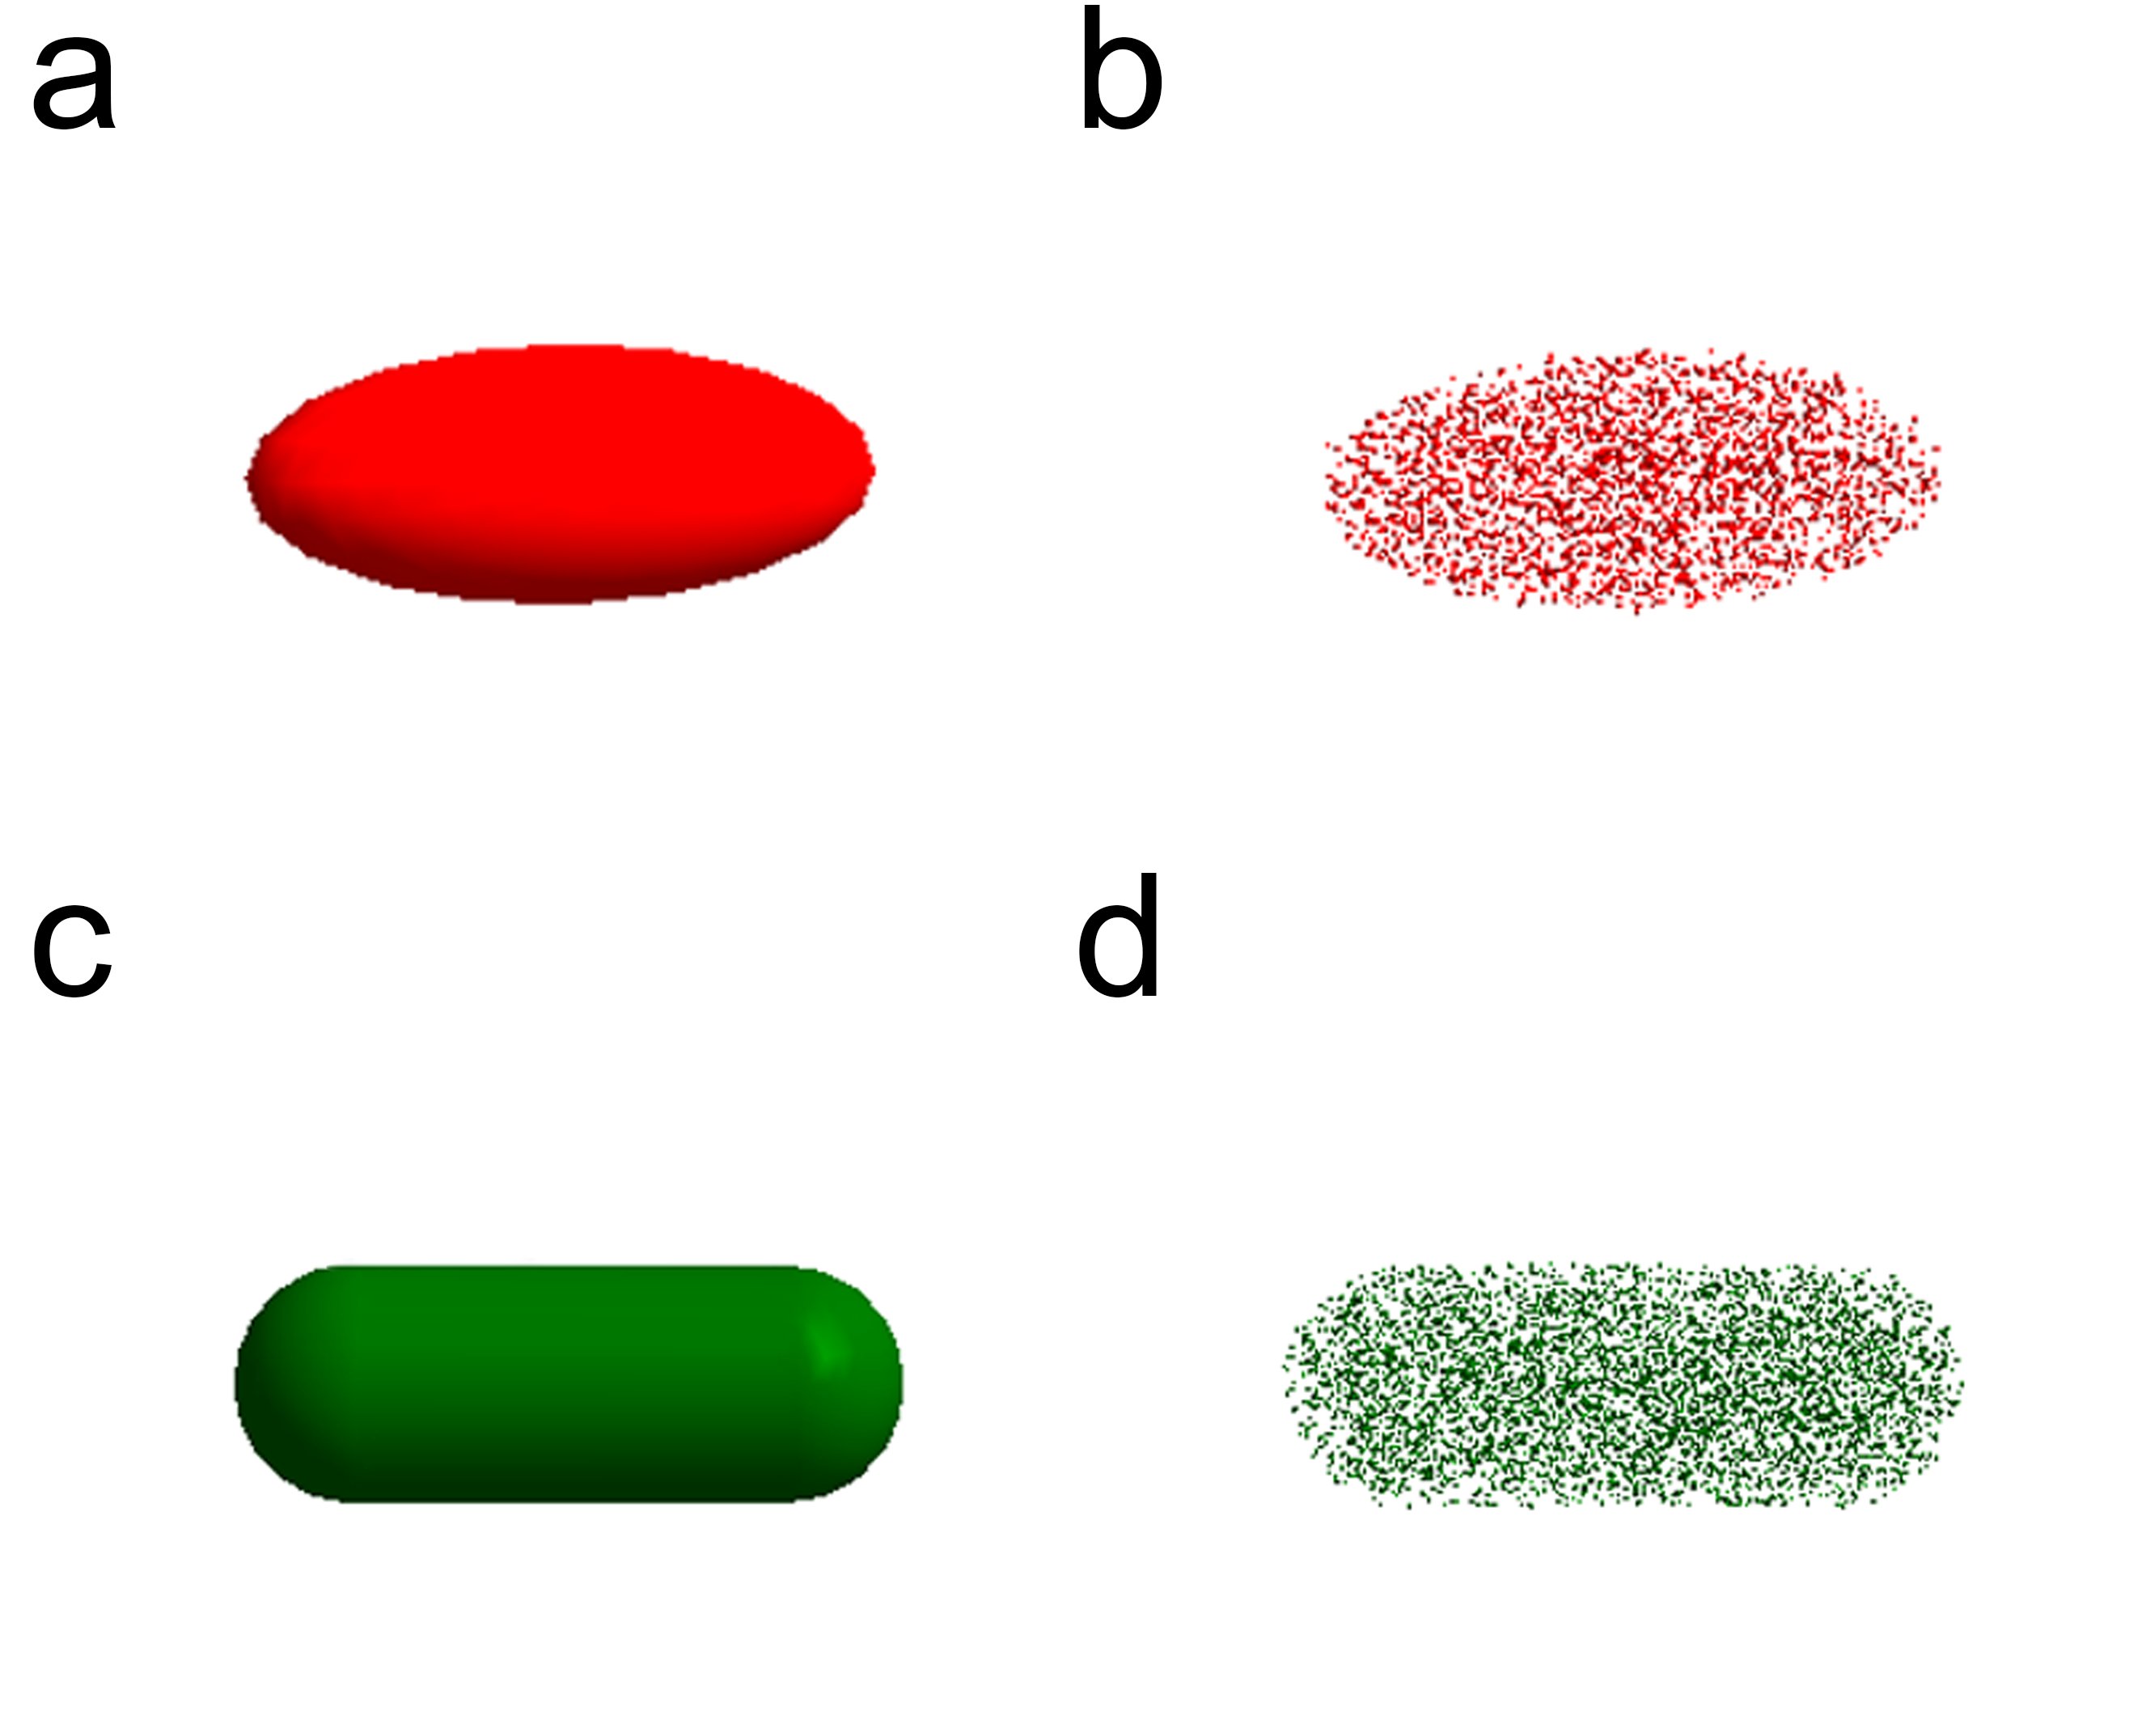
\includegraphics[width=0.5\columnwidth]{Scatteringmodel_single.png}
    \caption{Solid representations of a ellipsoid (a) and a spherocylinder (c). Mesh representations of a ellipsoid (b) and a spherocylinder (d).}
    \label{fig:scatt_mod_single}
\end{figure}

\begin{figure}
    \centering
    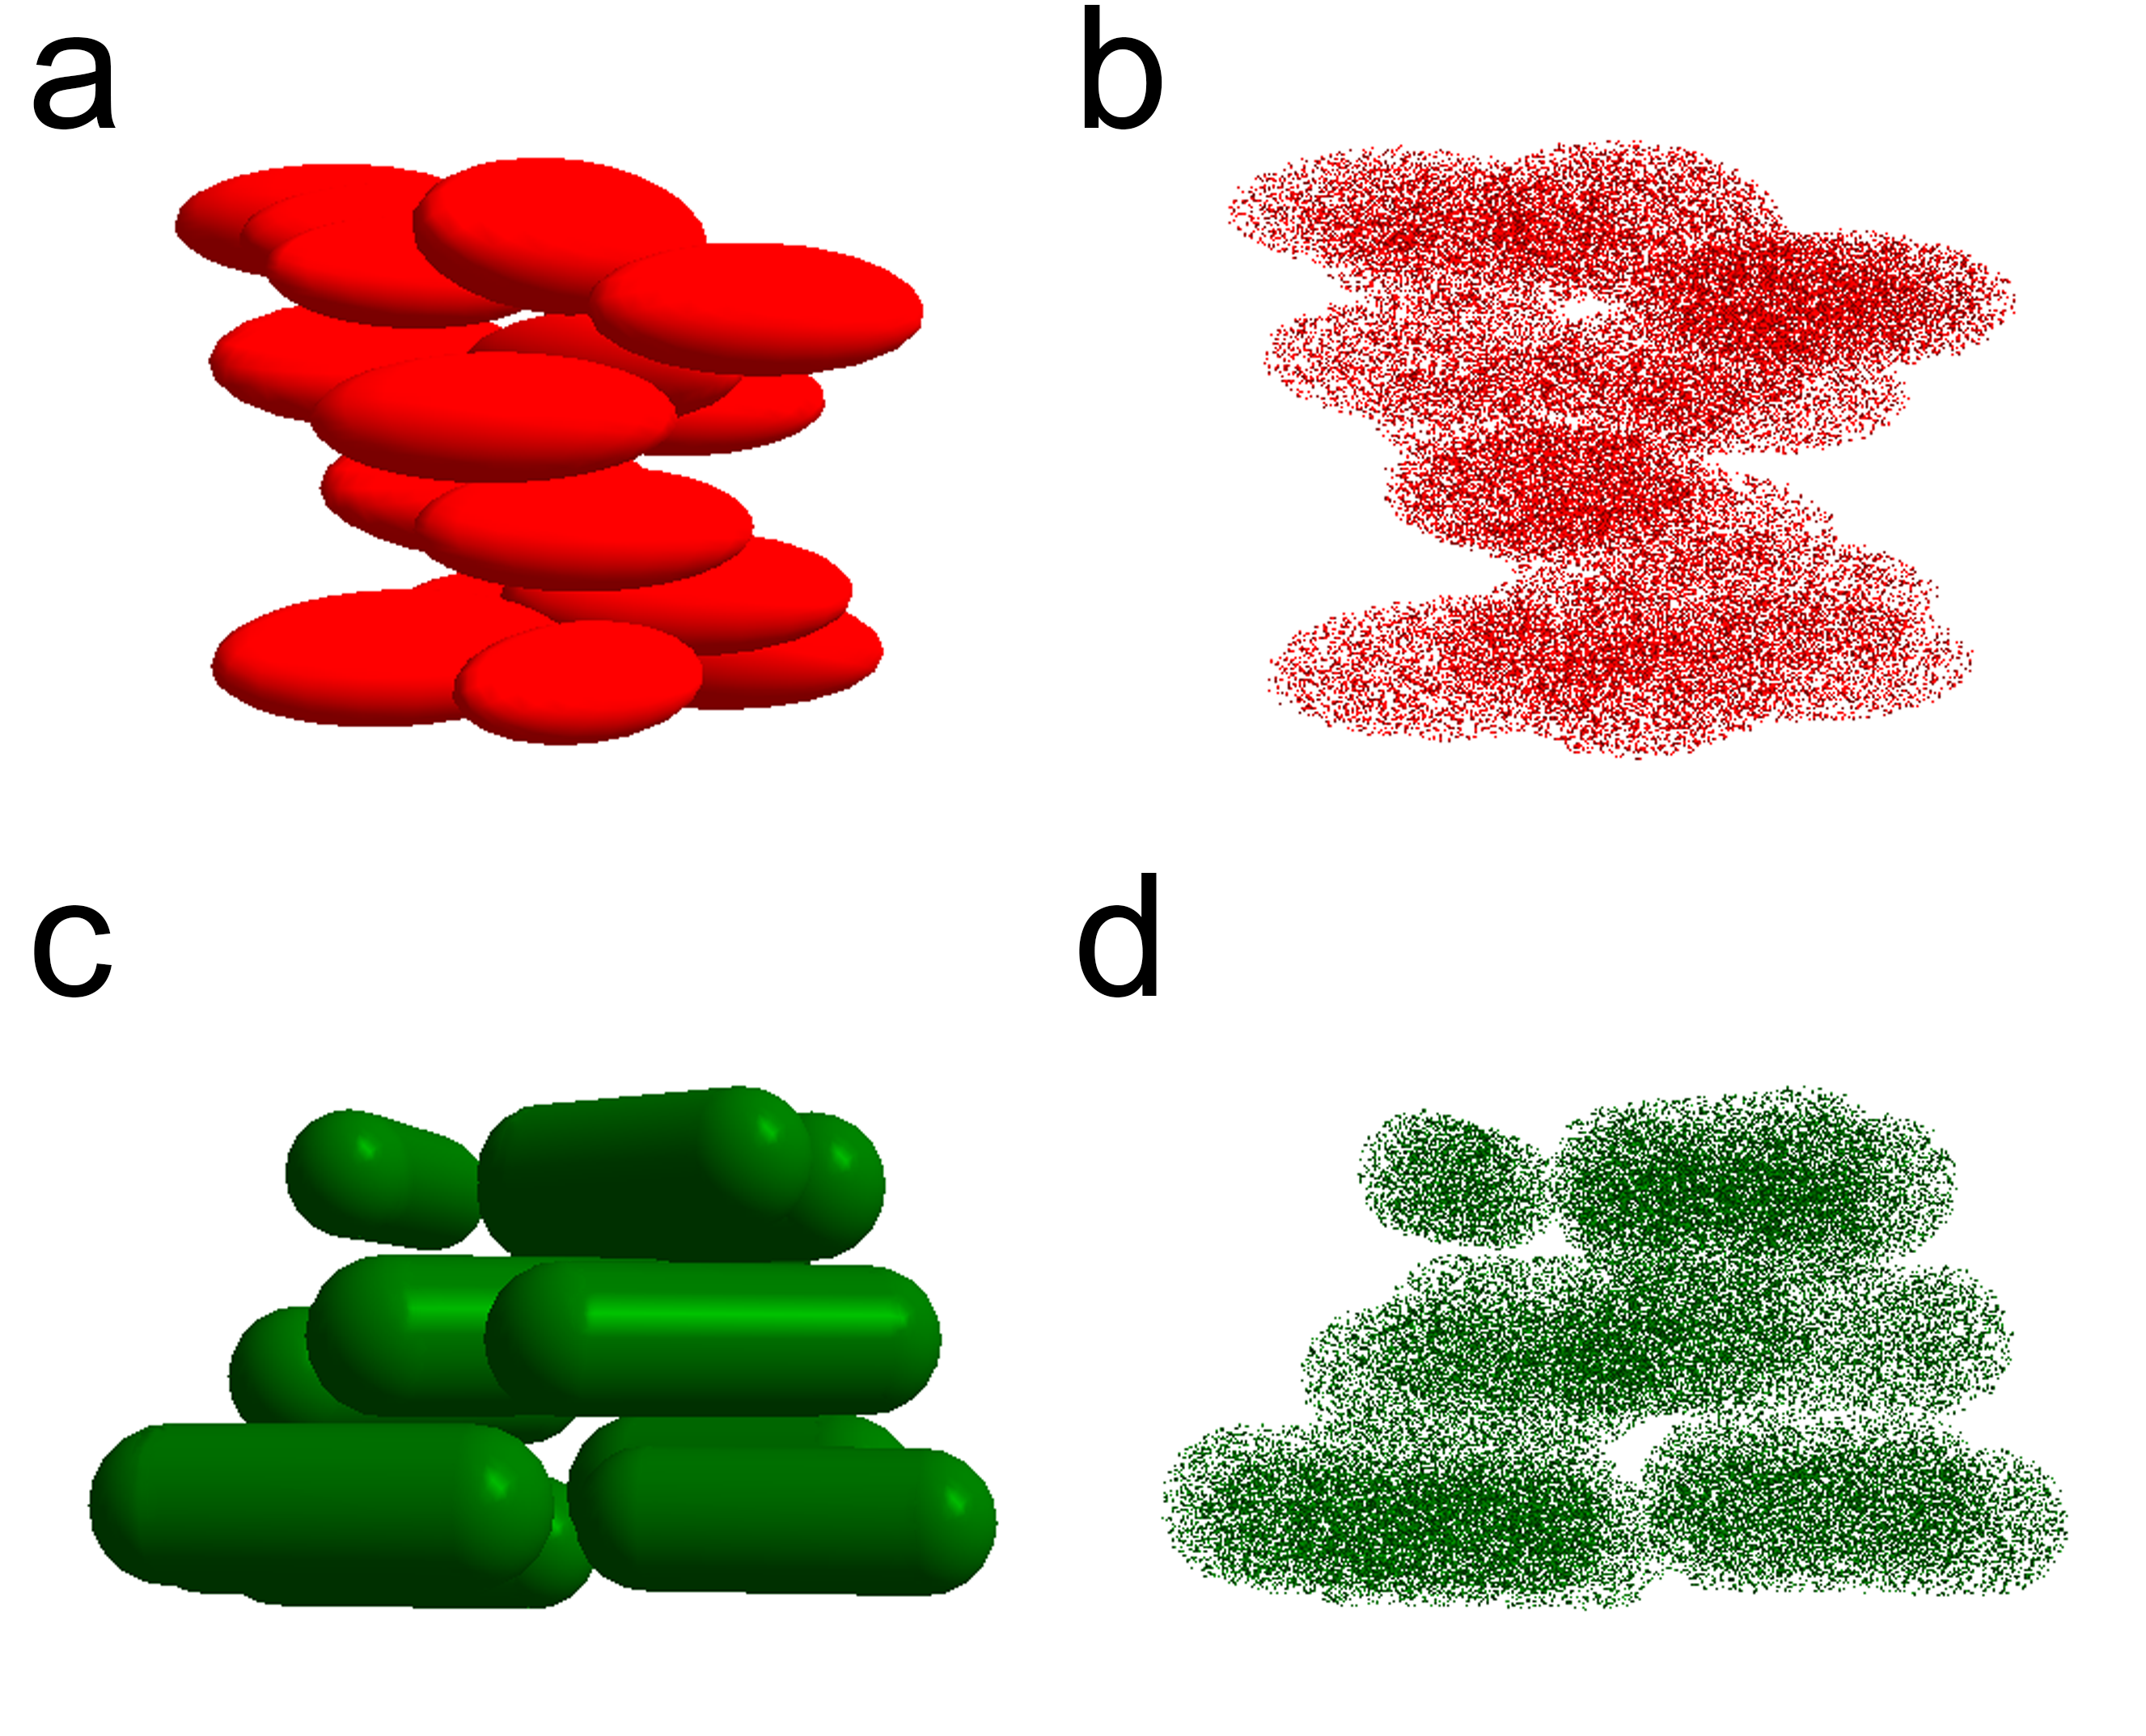
\includegraphics[width=0.5\columnwidth]{Scatteringmodel1.png}
    \caption{Example configurations for the structure factor calculation. Systems of ellipoids as solids (a) and meshes (b) and spherocylinders as solids (c) and meshes (d).}
    \label{fig:scatt_mod1}
\end{figure}


\begin{figure}
    \centering
    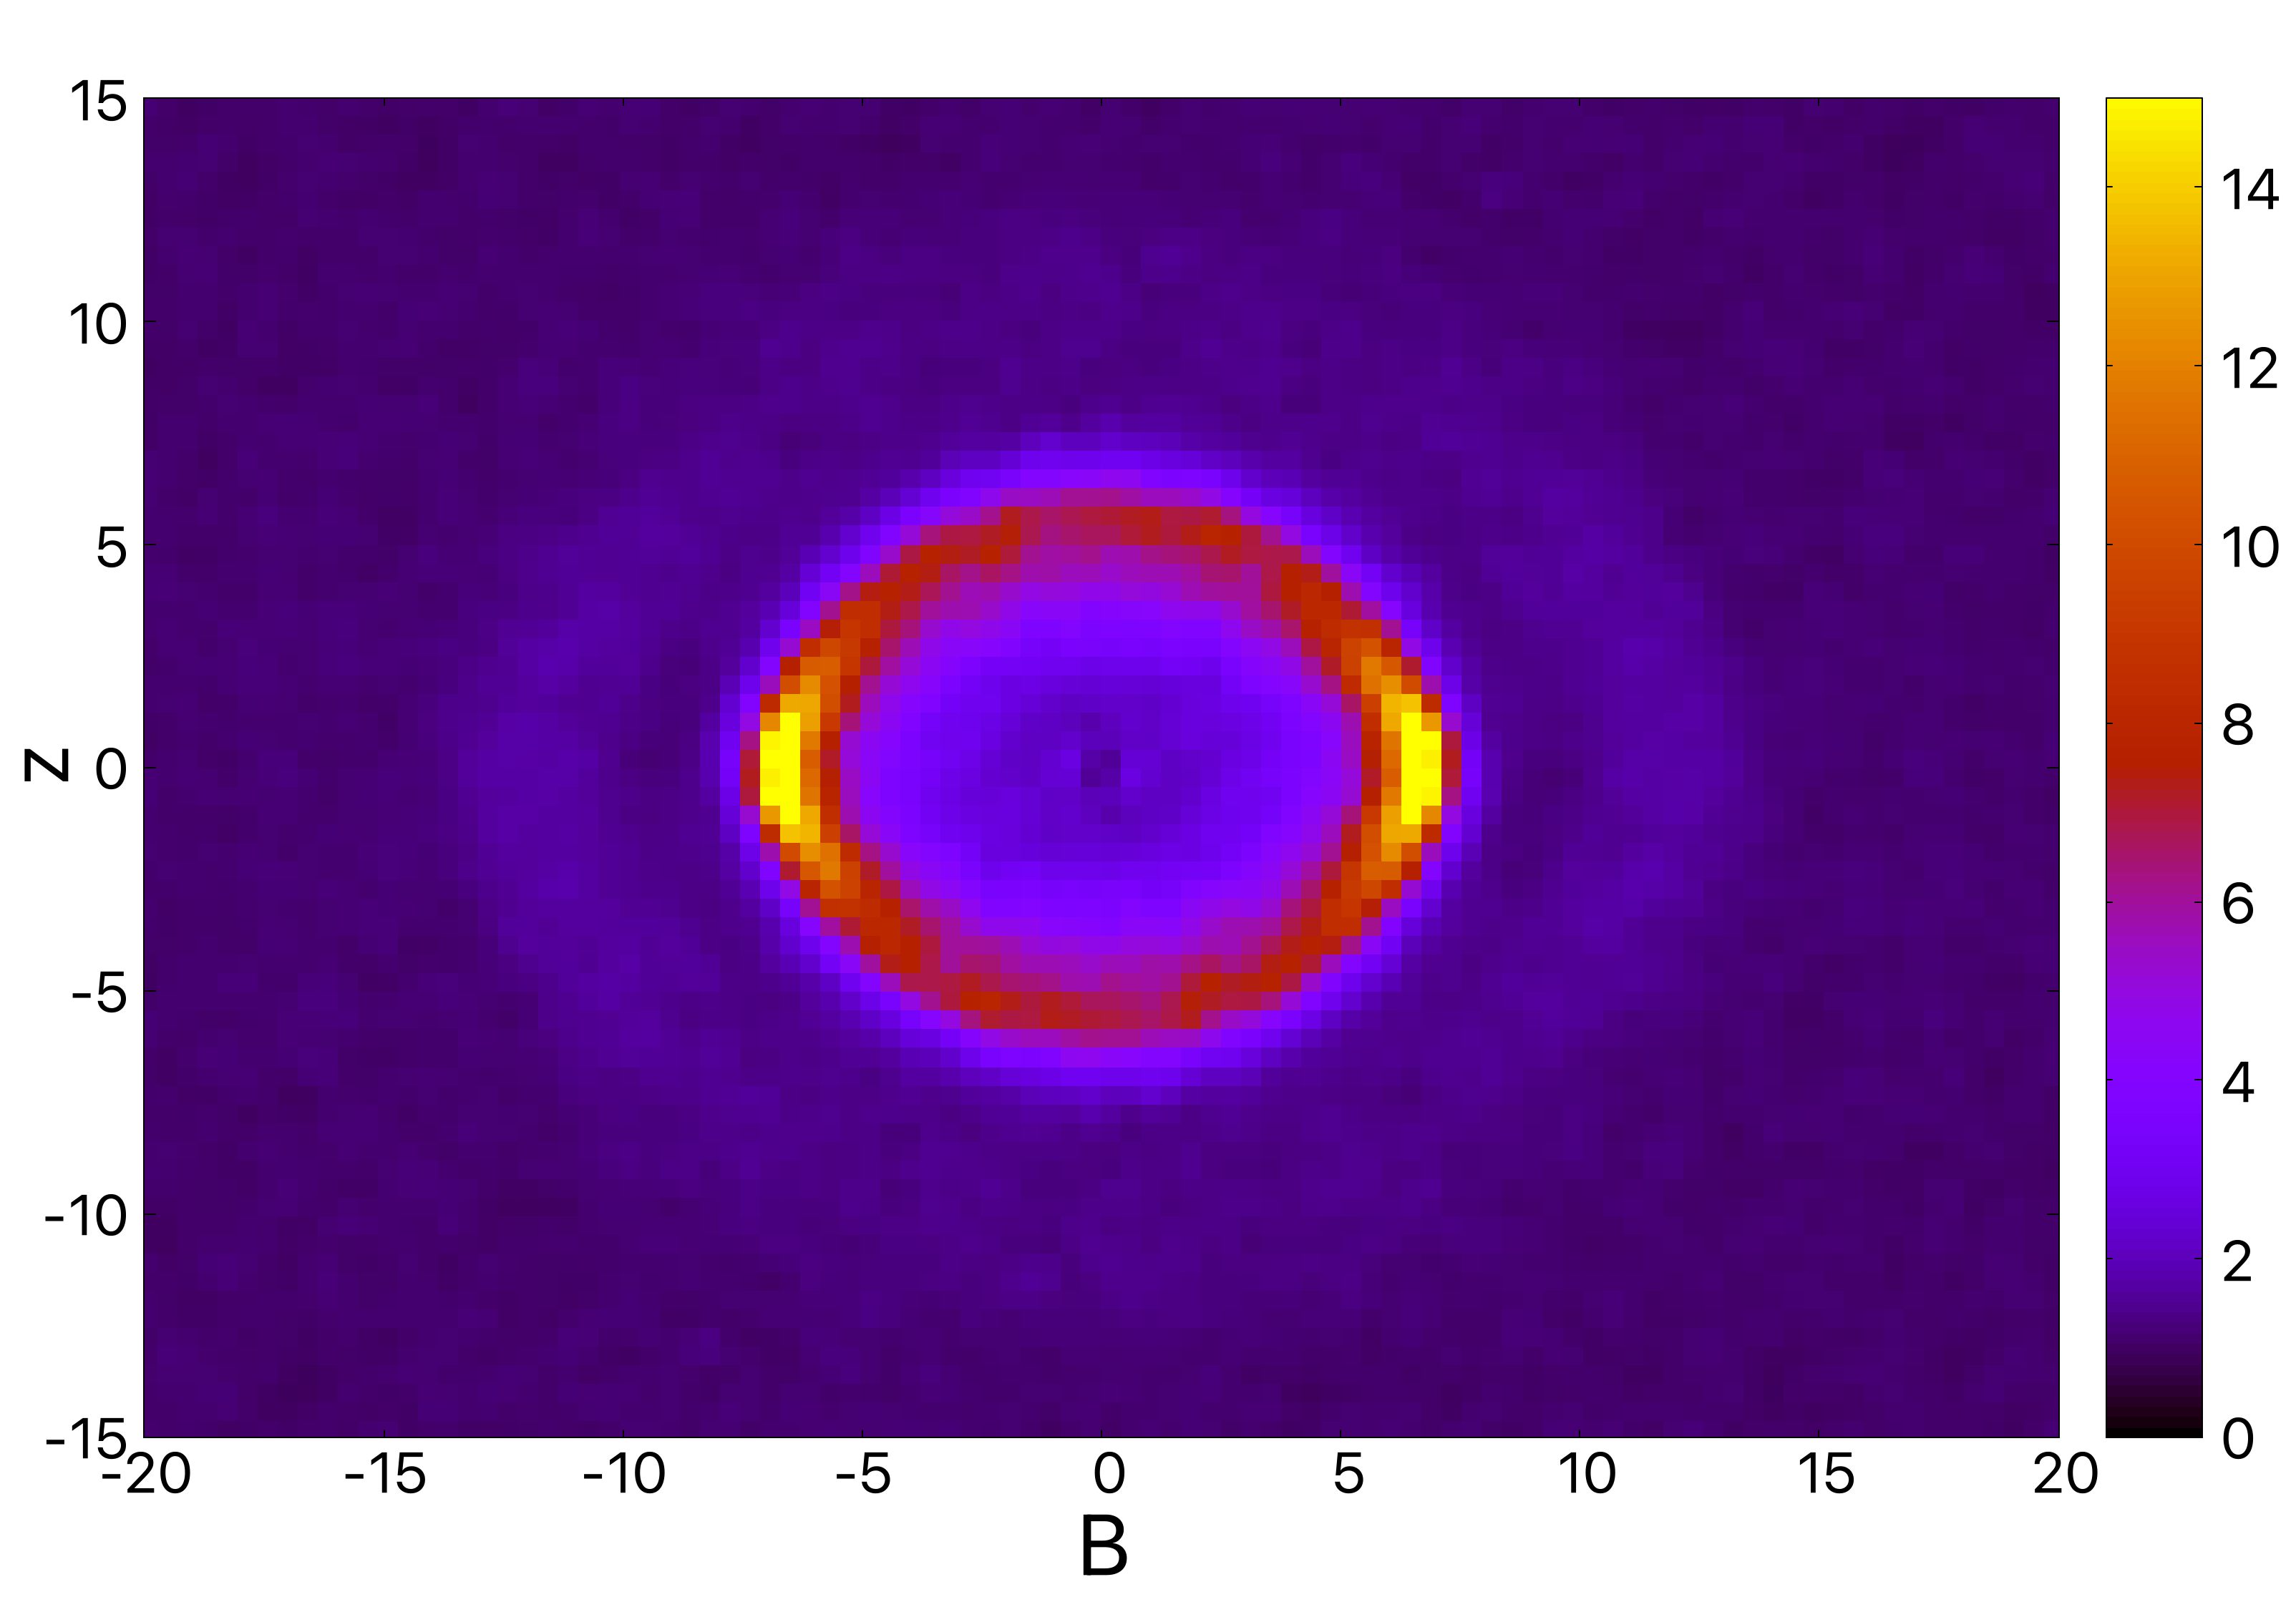
\includegraphics[width=0.7\columnwidth]{Syz_B_HE.png}
    \caption{Structure factor $S(0, q_y, q_z)$ of a system of hard ellipsoids with the presence of a magnetic field long the y axis at $\phi=0.50$.}
    \label{fig:Syz_B_HE}
\end{figure}

\begin{figure}
    \centering
    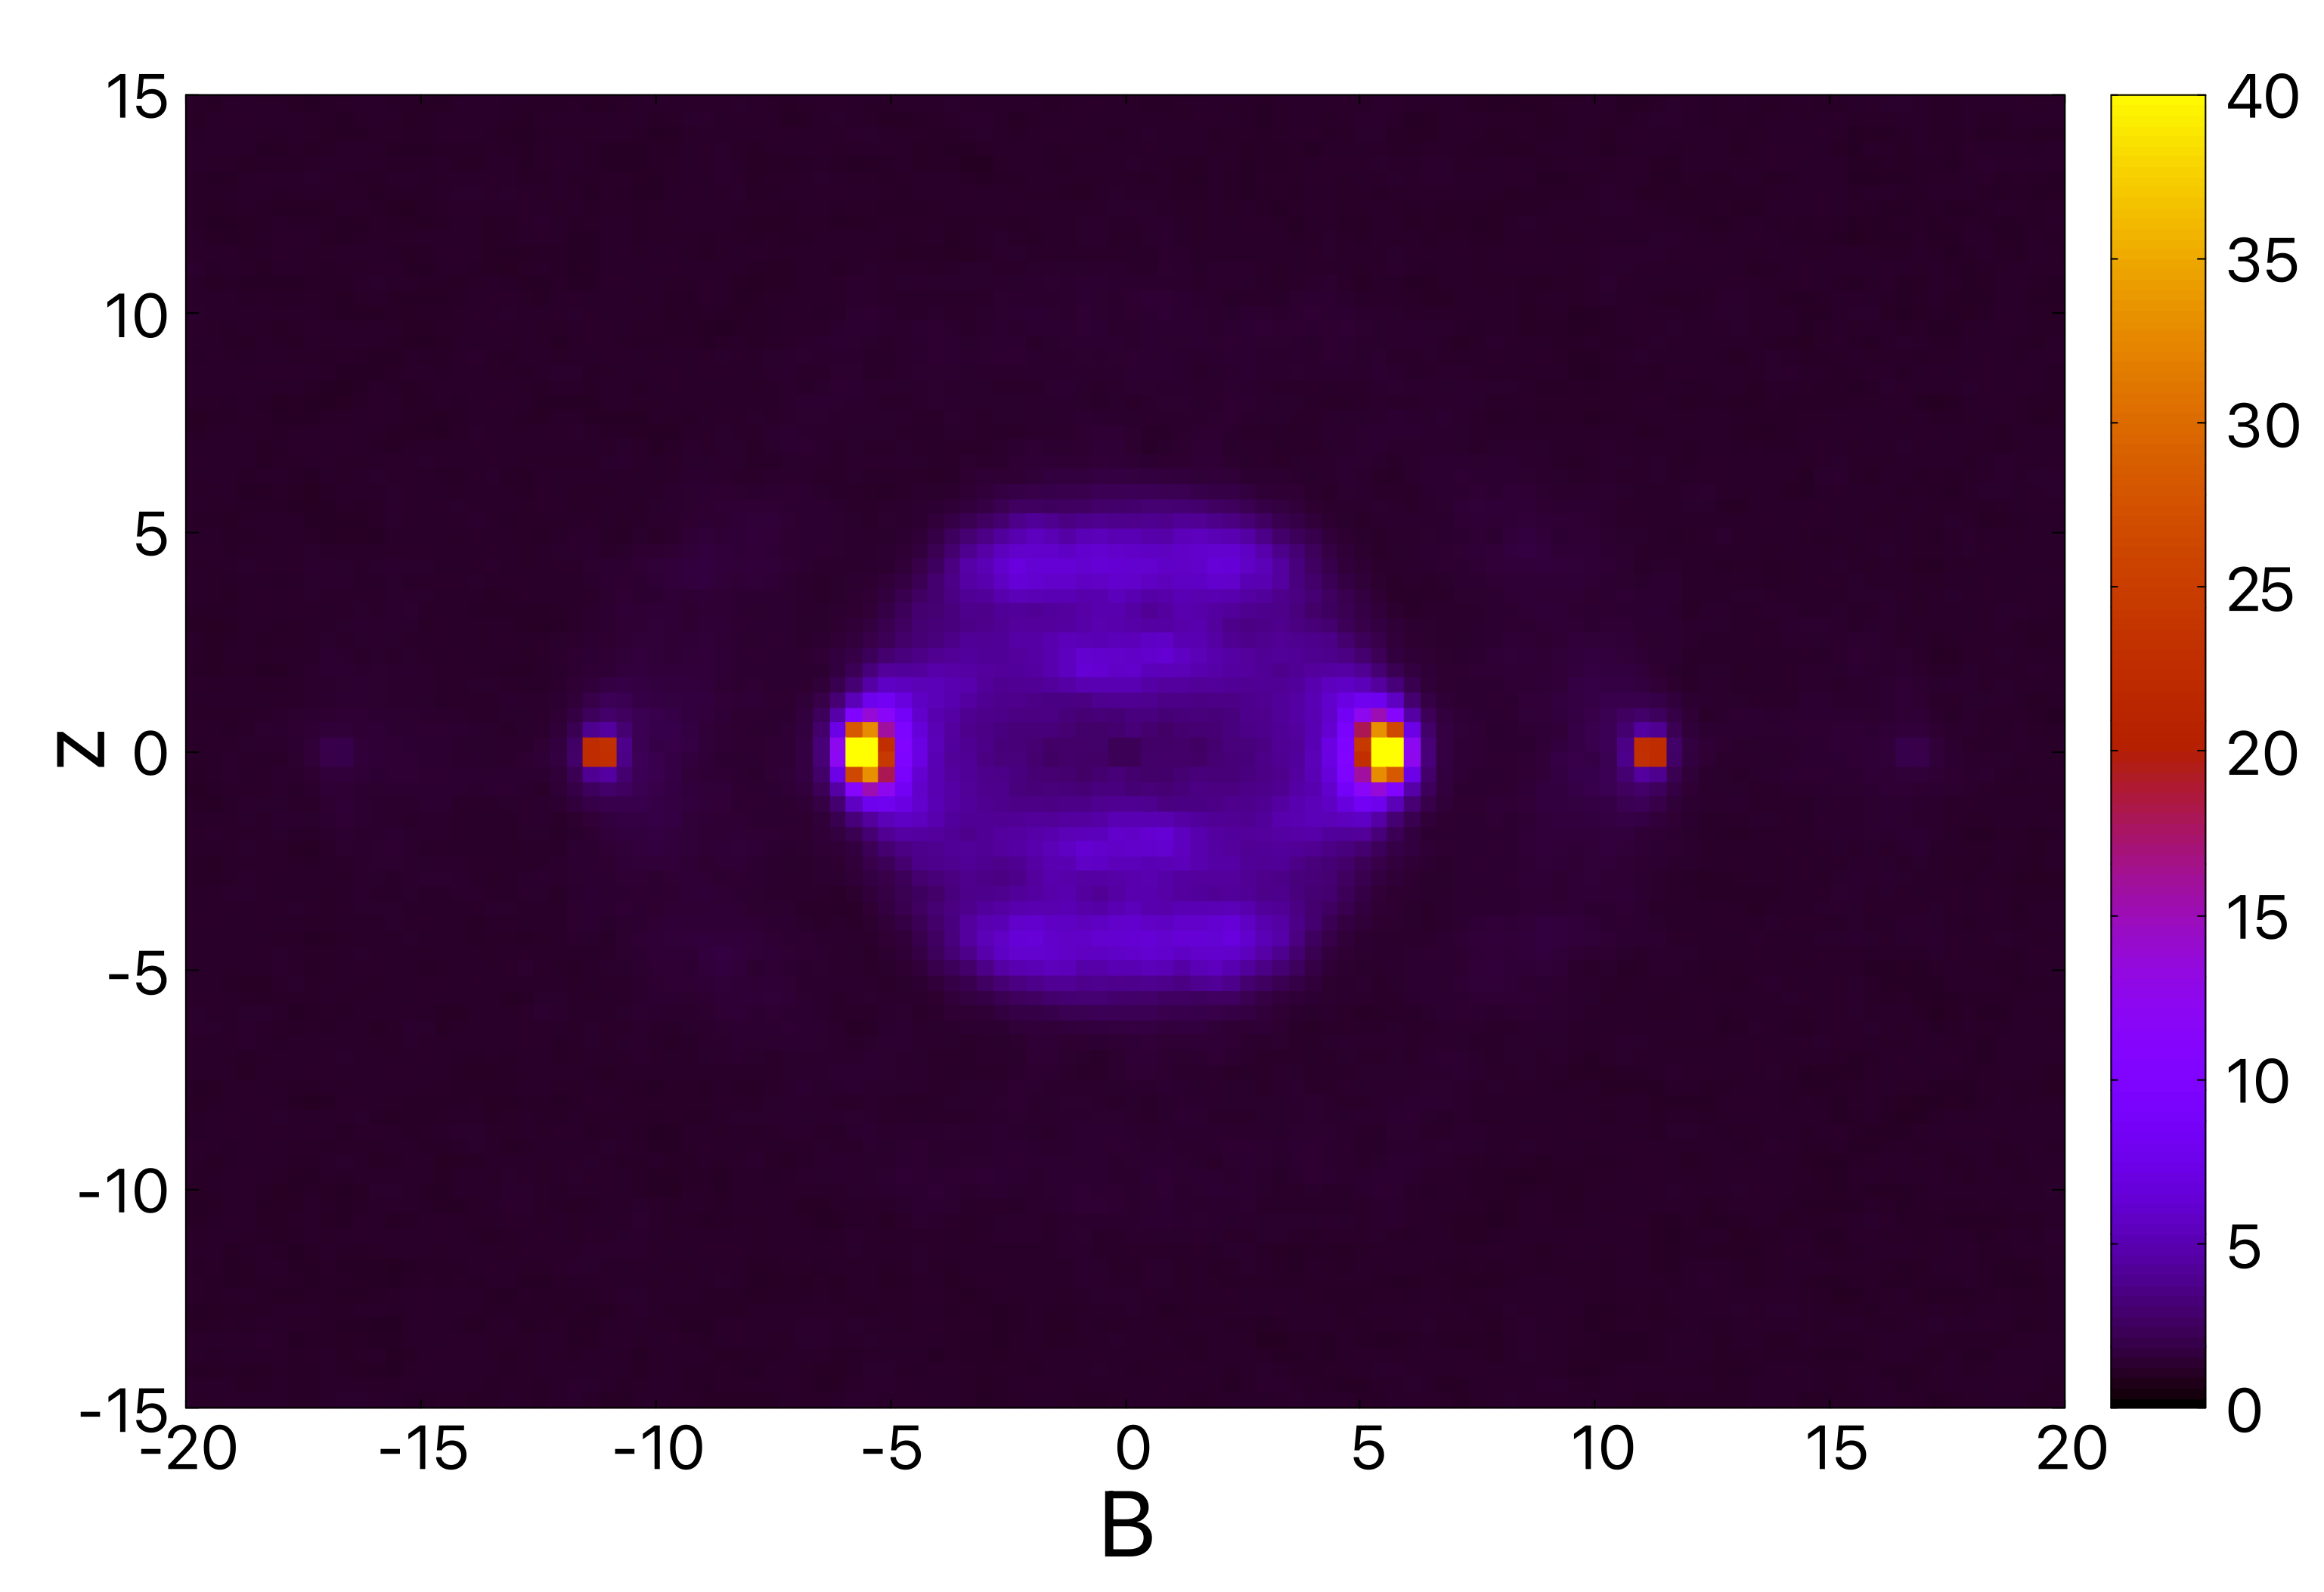
\includegraphics[width=0.7\columnwidth]{Syz_B.png}
    \caption{Structure factor $S(0, q_y, q_z)$ of a system of spherocylinders with the presence of a magnetic field long the y axis at $\phi=0.50$.}
    \label{fig:Syz_B_HSC}
\end{figure}

\subsection{Pair distribution function}

The spatial characterization of the phases can be further analyzed by  the calculation of the three-dimensional pair distribution function $g(\vec{r})$:

\begin{equation}
    g(\vec{r}) = \frac{1}{\rho N} \left\langle \sum_{i=1}^N \sum_{j\neq i} \delta \left( \vec{r} - \left( \vec{r}_i - \vec{r}_j \right) \right) \right\rangle
\end{equation}

where $\delta(x)$ is the Dirac delta function. This quantity has been calculated averaging on the same configurations used for the structure factor \ref{eq:S_q}, obtaining the pair distribution function on a plane parallel to the magnetic field $yz$ and on the perpendicular plane $xz$. The results are represented in Fig. \ref{fig:gyz_B} and Fig. \ref{fig:gxz_B}. The smectic phase is evident: it can be noticed the different planes along the y axis (Fig. \ref{fig:gyz_B}) and the 2D liquid behaviour in-plane (Fig. \ref{fig:gxz_B}).
Differently the radial distribution function of HEs does not show any layering for all state points studies.
A typical example of $g(r)$ for HEs is shown in Fig.\ref{fig:gyz_B_HE} (yz-plane) and Fig.~\ref{fig:gxz_B_HE} (xz-plane). The anisotropy and structuring shown in Fig.\ref{fig:gyz_B_HE} reflect the alignment of HEs due
to the magnetic field. Differently, the anisotropy of the radial distribution function calculated
onto a plane perpendicular to the magnetic field, which is shown in Fig.~\ref{fig:gxz_B_HE}, is due to 
orientational ordering of HEs, which builds up at volume fraction higher than $\approx 0.45$. 
More details on this are provided below (see Section ``Smectic and nematic ordering'').

\begin{figure}
    \begin{center}
    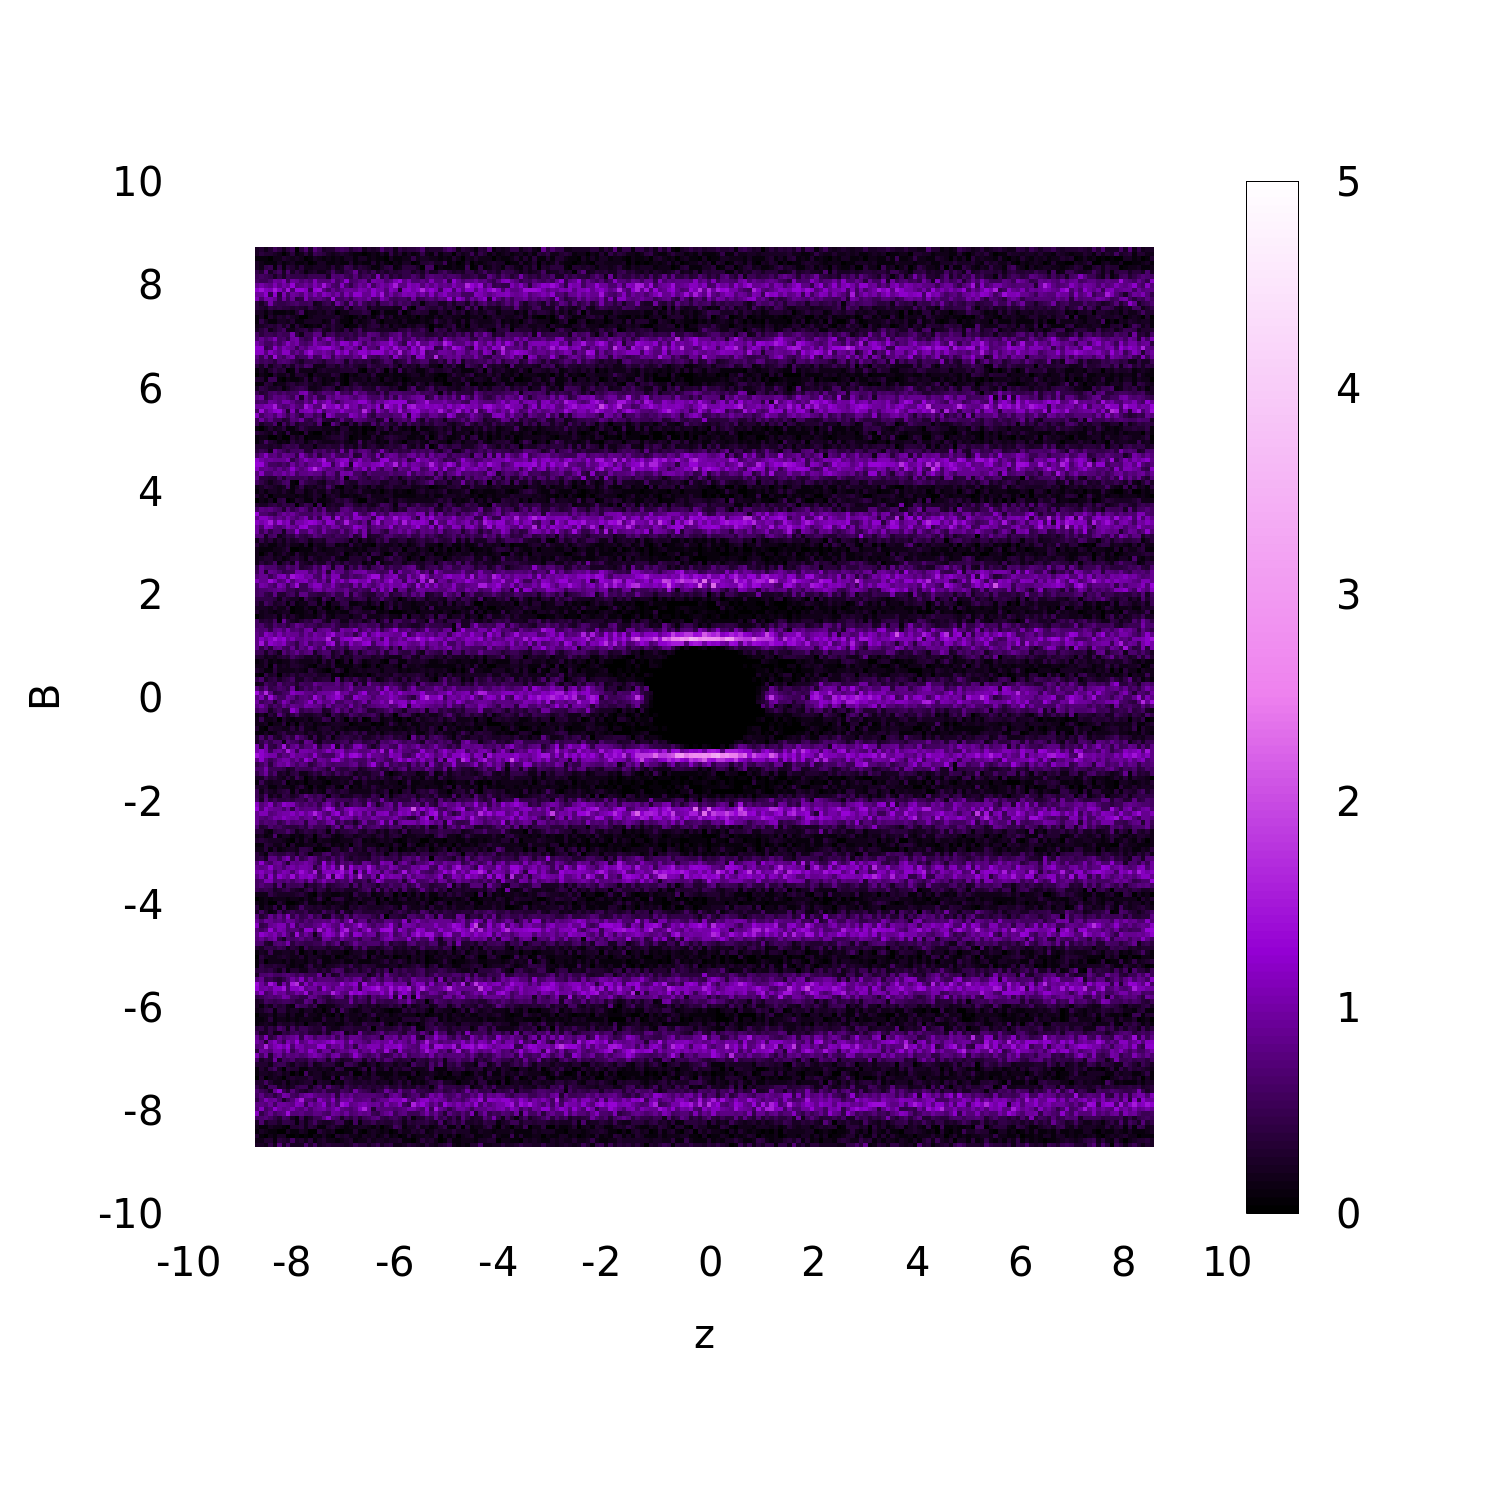
\includegraphics[width=0.7\columnwidth]{gyz_B.png}
    \caption{Pair distribution function for a system of spherocylinders $\phi = 0.50$ in presence of a magnetic field $\vec{B}$ along y axis.}
    \label{fig:gyz_B}
    \end{center}
\end{figure}


\begin{figure}
    \centering
    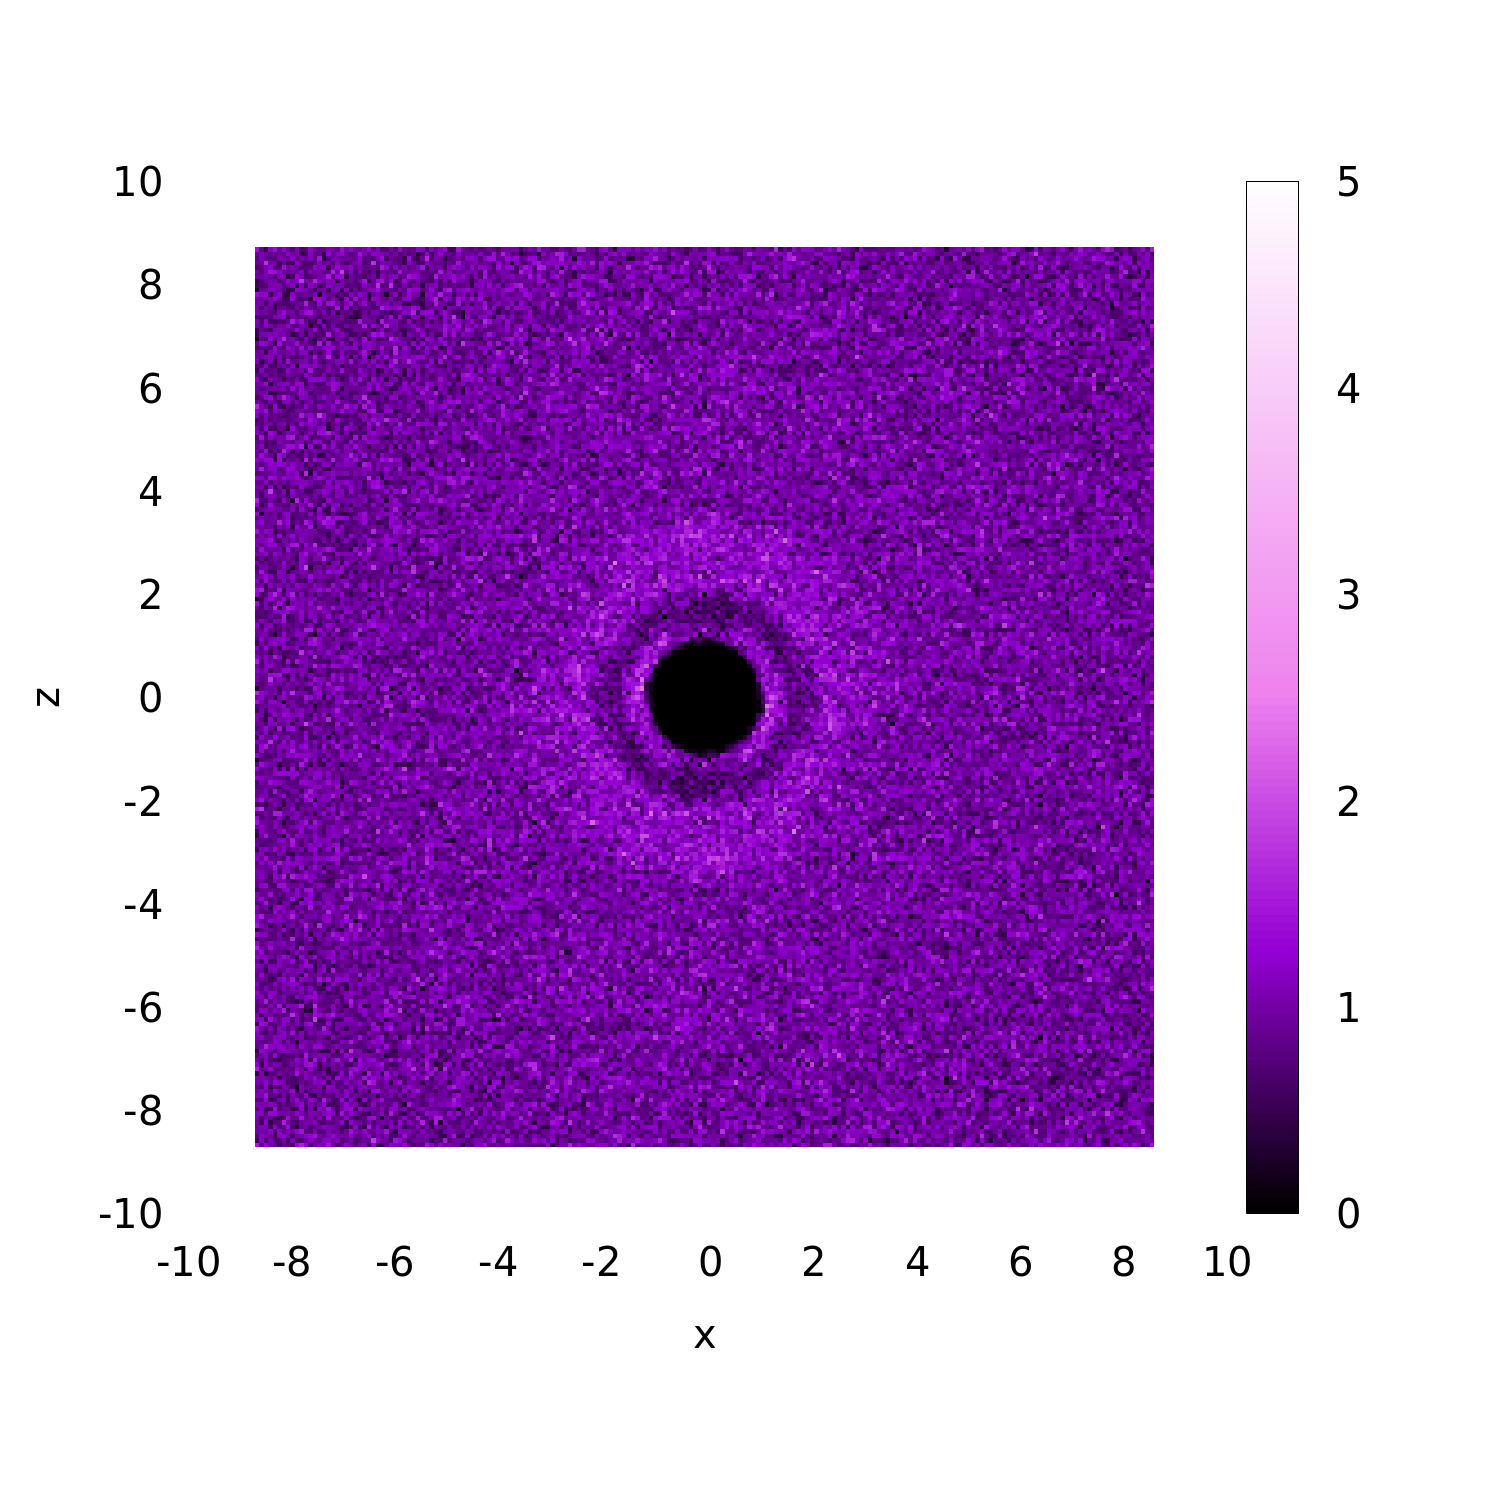
\includegraphics[width=0.8\columnwidth]{gxz_B.png}
    \caption{Pair distribution function for a system of spherocylinders $\phi = 0.50$ in presence of a magnetic field $\vec{B}$ along y axis.}
    \label{fig:gxz_B}
\end{figure}

\begin{figure}
    \begin{center}
    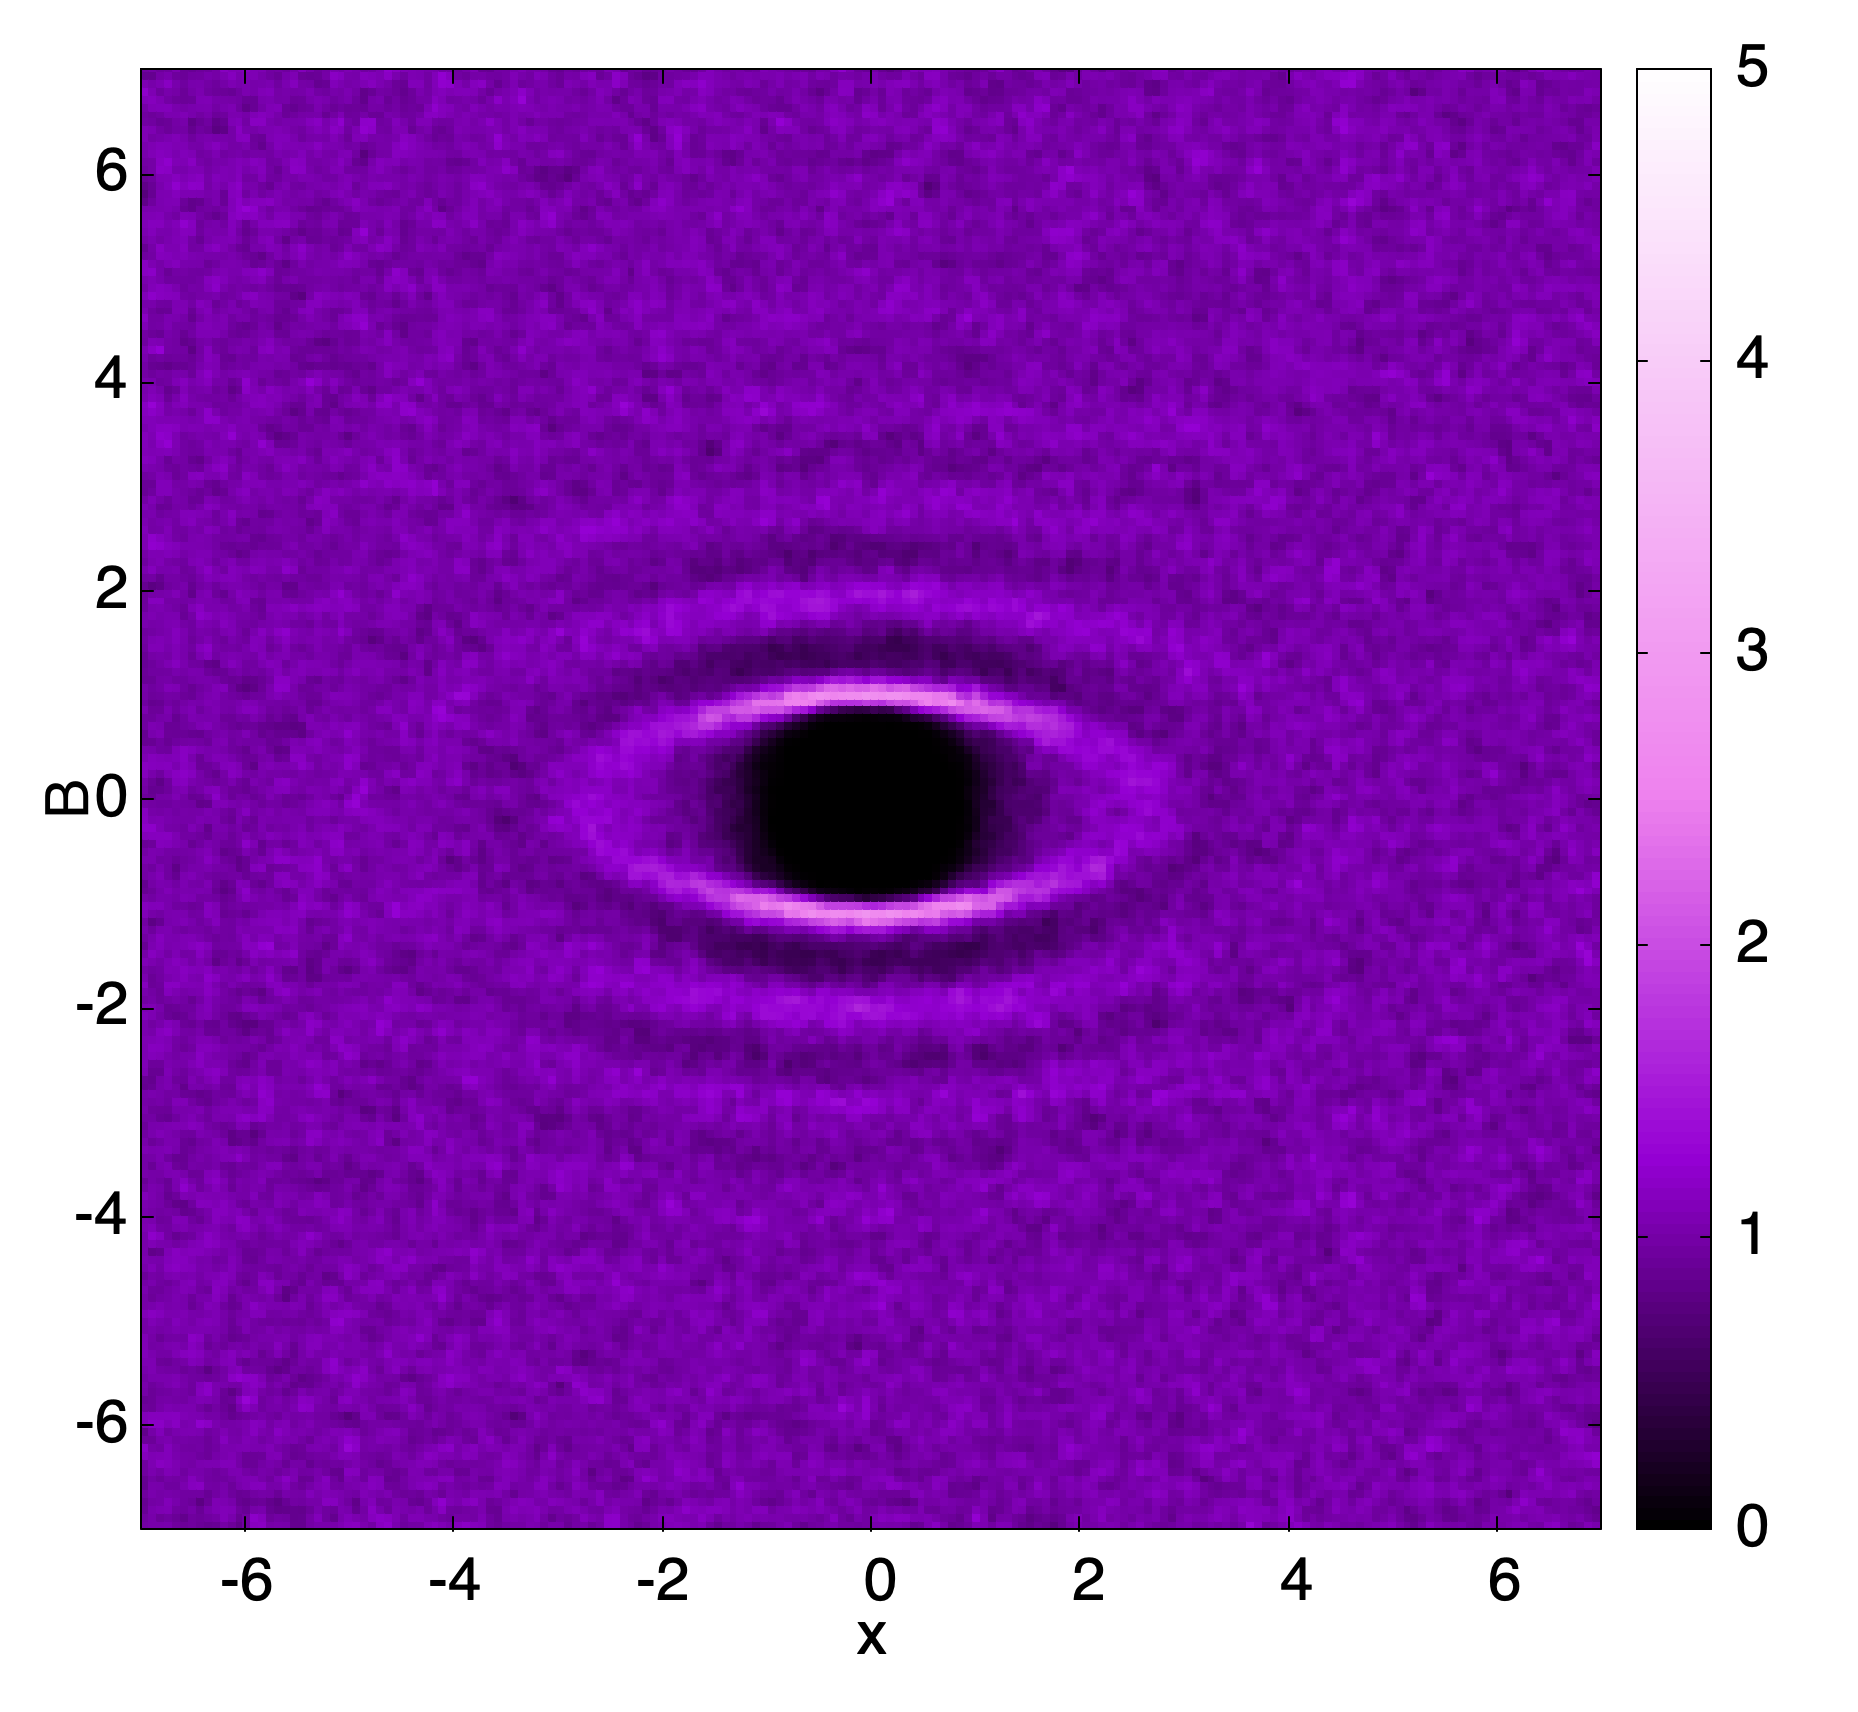
\includegraphics[width=0.7\columnwidth]{gyz_B_HE.png}
    \caption{Pair distribution function for a system of hard ellipsoids at $\phi = 0.50$ in presence of a magnetic field $\vec{B}$ along y axis.}
    \label{fig:gyz_B_HE}
    \end{center}
\end{figure}


\begin{figure}
    \centering
    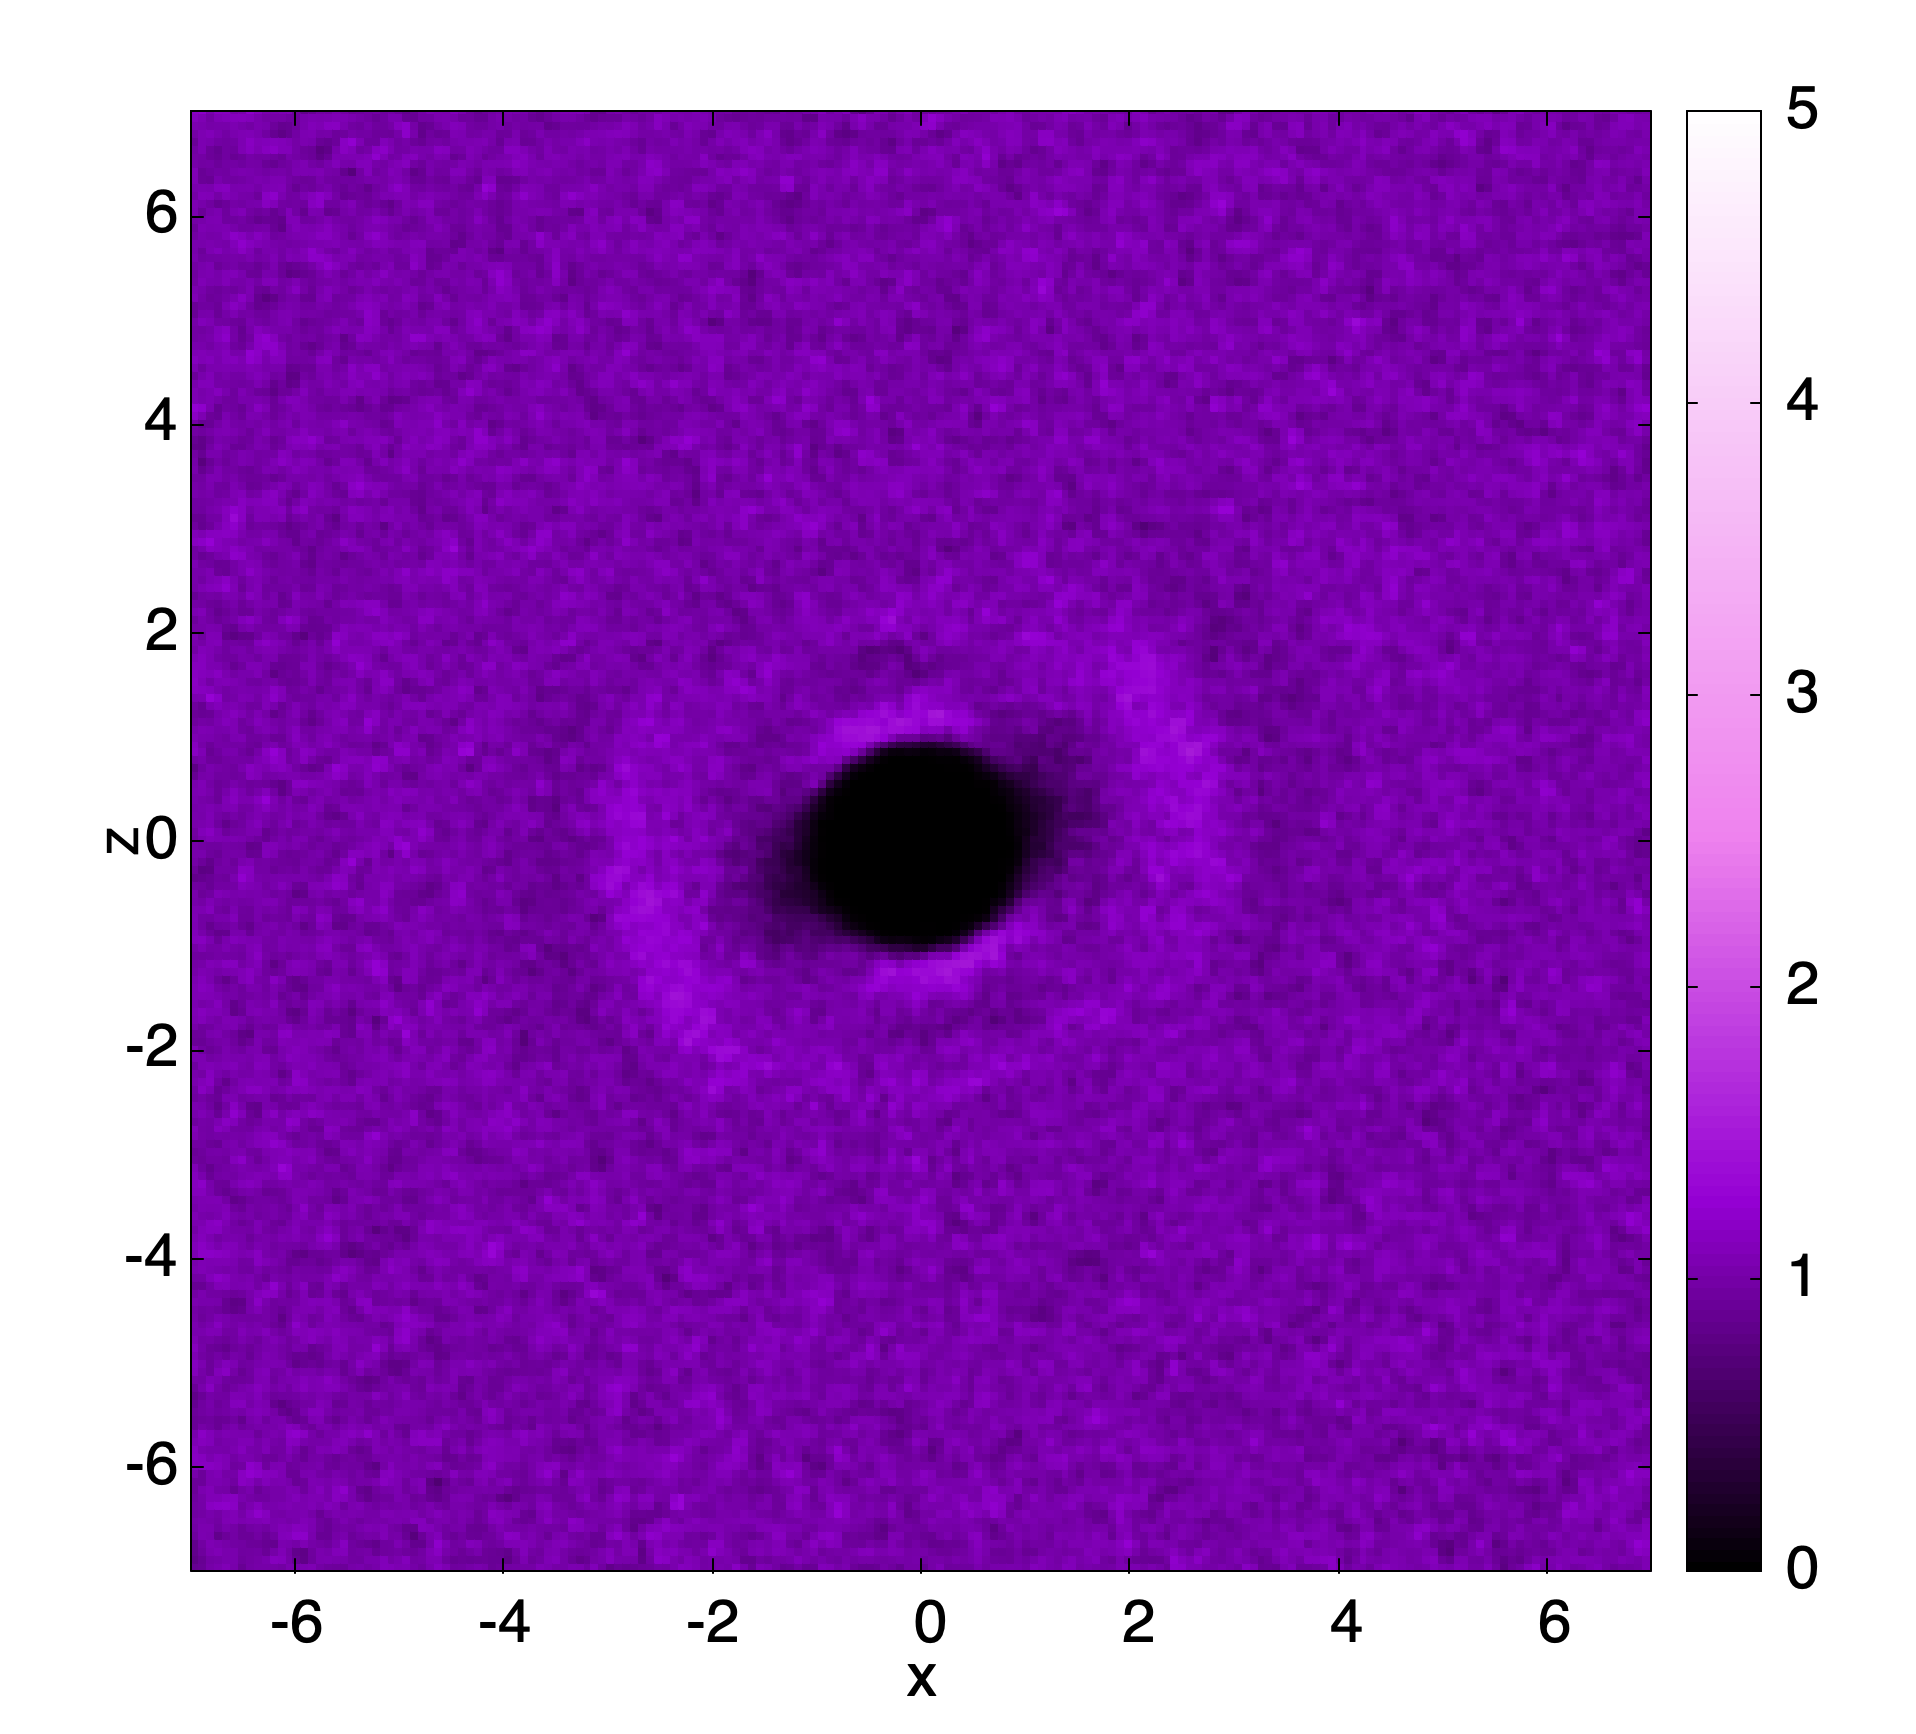
\includegraphics[width=0.7\columnwidth]{gxz_B_HE.png}
    \caption{Pair distribution function for a system of hard ellipsoids at $\phi = 0.50$ in presence of a magnetic field $\vec{B}$ along y axis.}
    \label{fig:gxz_B_HE}
\end{figure}
%\newpage %usato solo per non far andare l'immagine prima

\section{Absence of magnetic field}

In order to demonstrate the magnetic origin of the smectic phase in these systems, we performed a Monte Carlo simulation in the NVT ensemble of a smectic configuration of spherocylinders with $\phi = 0.50$. As represented in Fig. \ref{fig:noB_snapshot}, in absence of a magnetic field the system preferentially arranges in a isotropic phase.

\subsection{Structure factor}
To further confirm the isotropy of this phase, it has been calculated the structure factor $S(0, q_y, q_z)$ of the system which presents a typical isotropic pattern (Fig. \ref{fig:Syz_noB}).

%\newpage    %da togliere

\begin{figure}
    \centering
    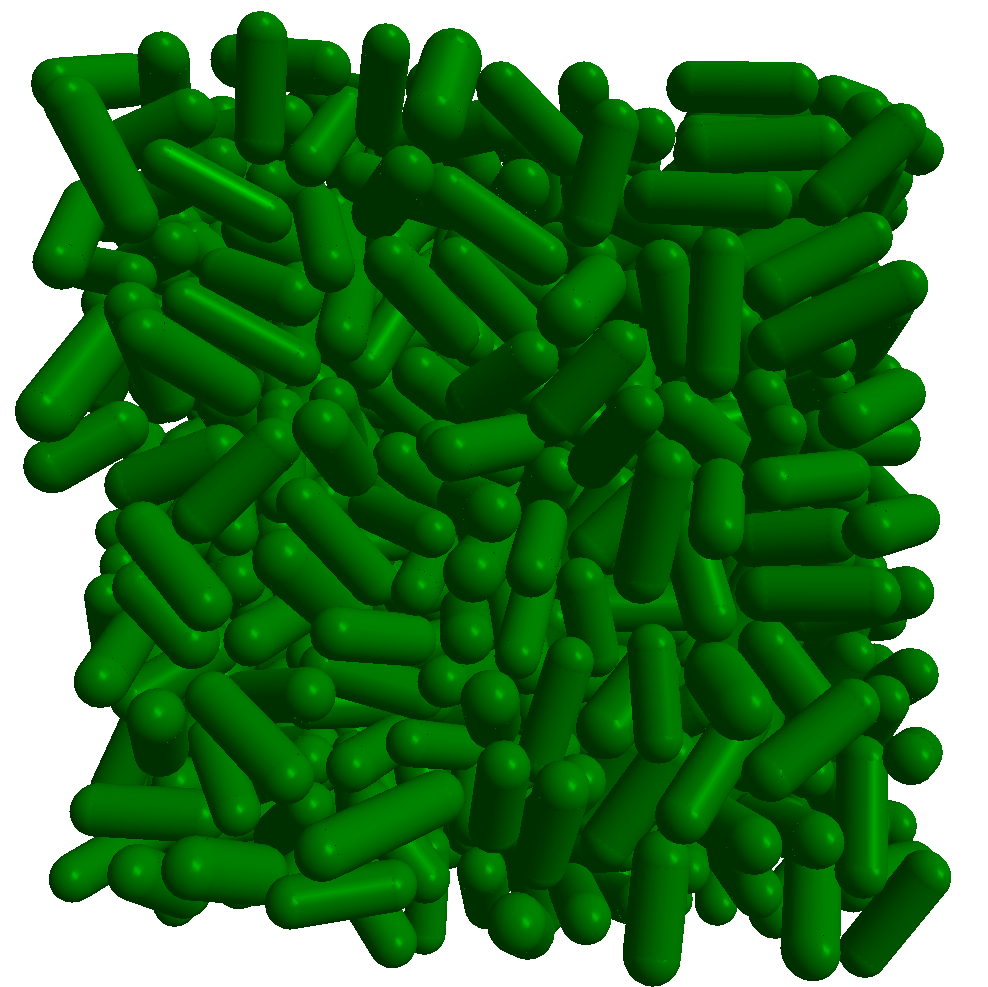
\includegraphics[width=0.5\columnwidth]{Isotropic_phase_snap.png}
    \caption{Snapshot of a system of polydisperse spherocylinders with $\phi = 0.50$ in absence of magnetic field.}
    \label{fig:noB_snapshot}
\end{figure}

\begin{figure}
    \centering
    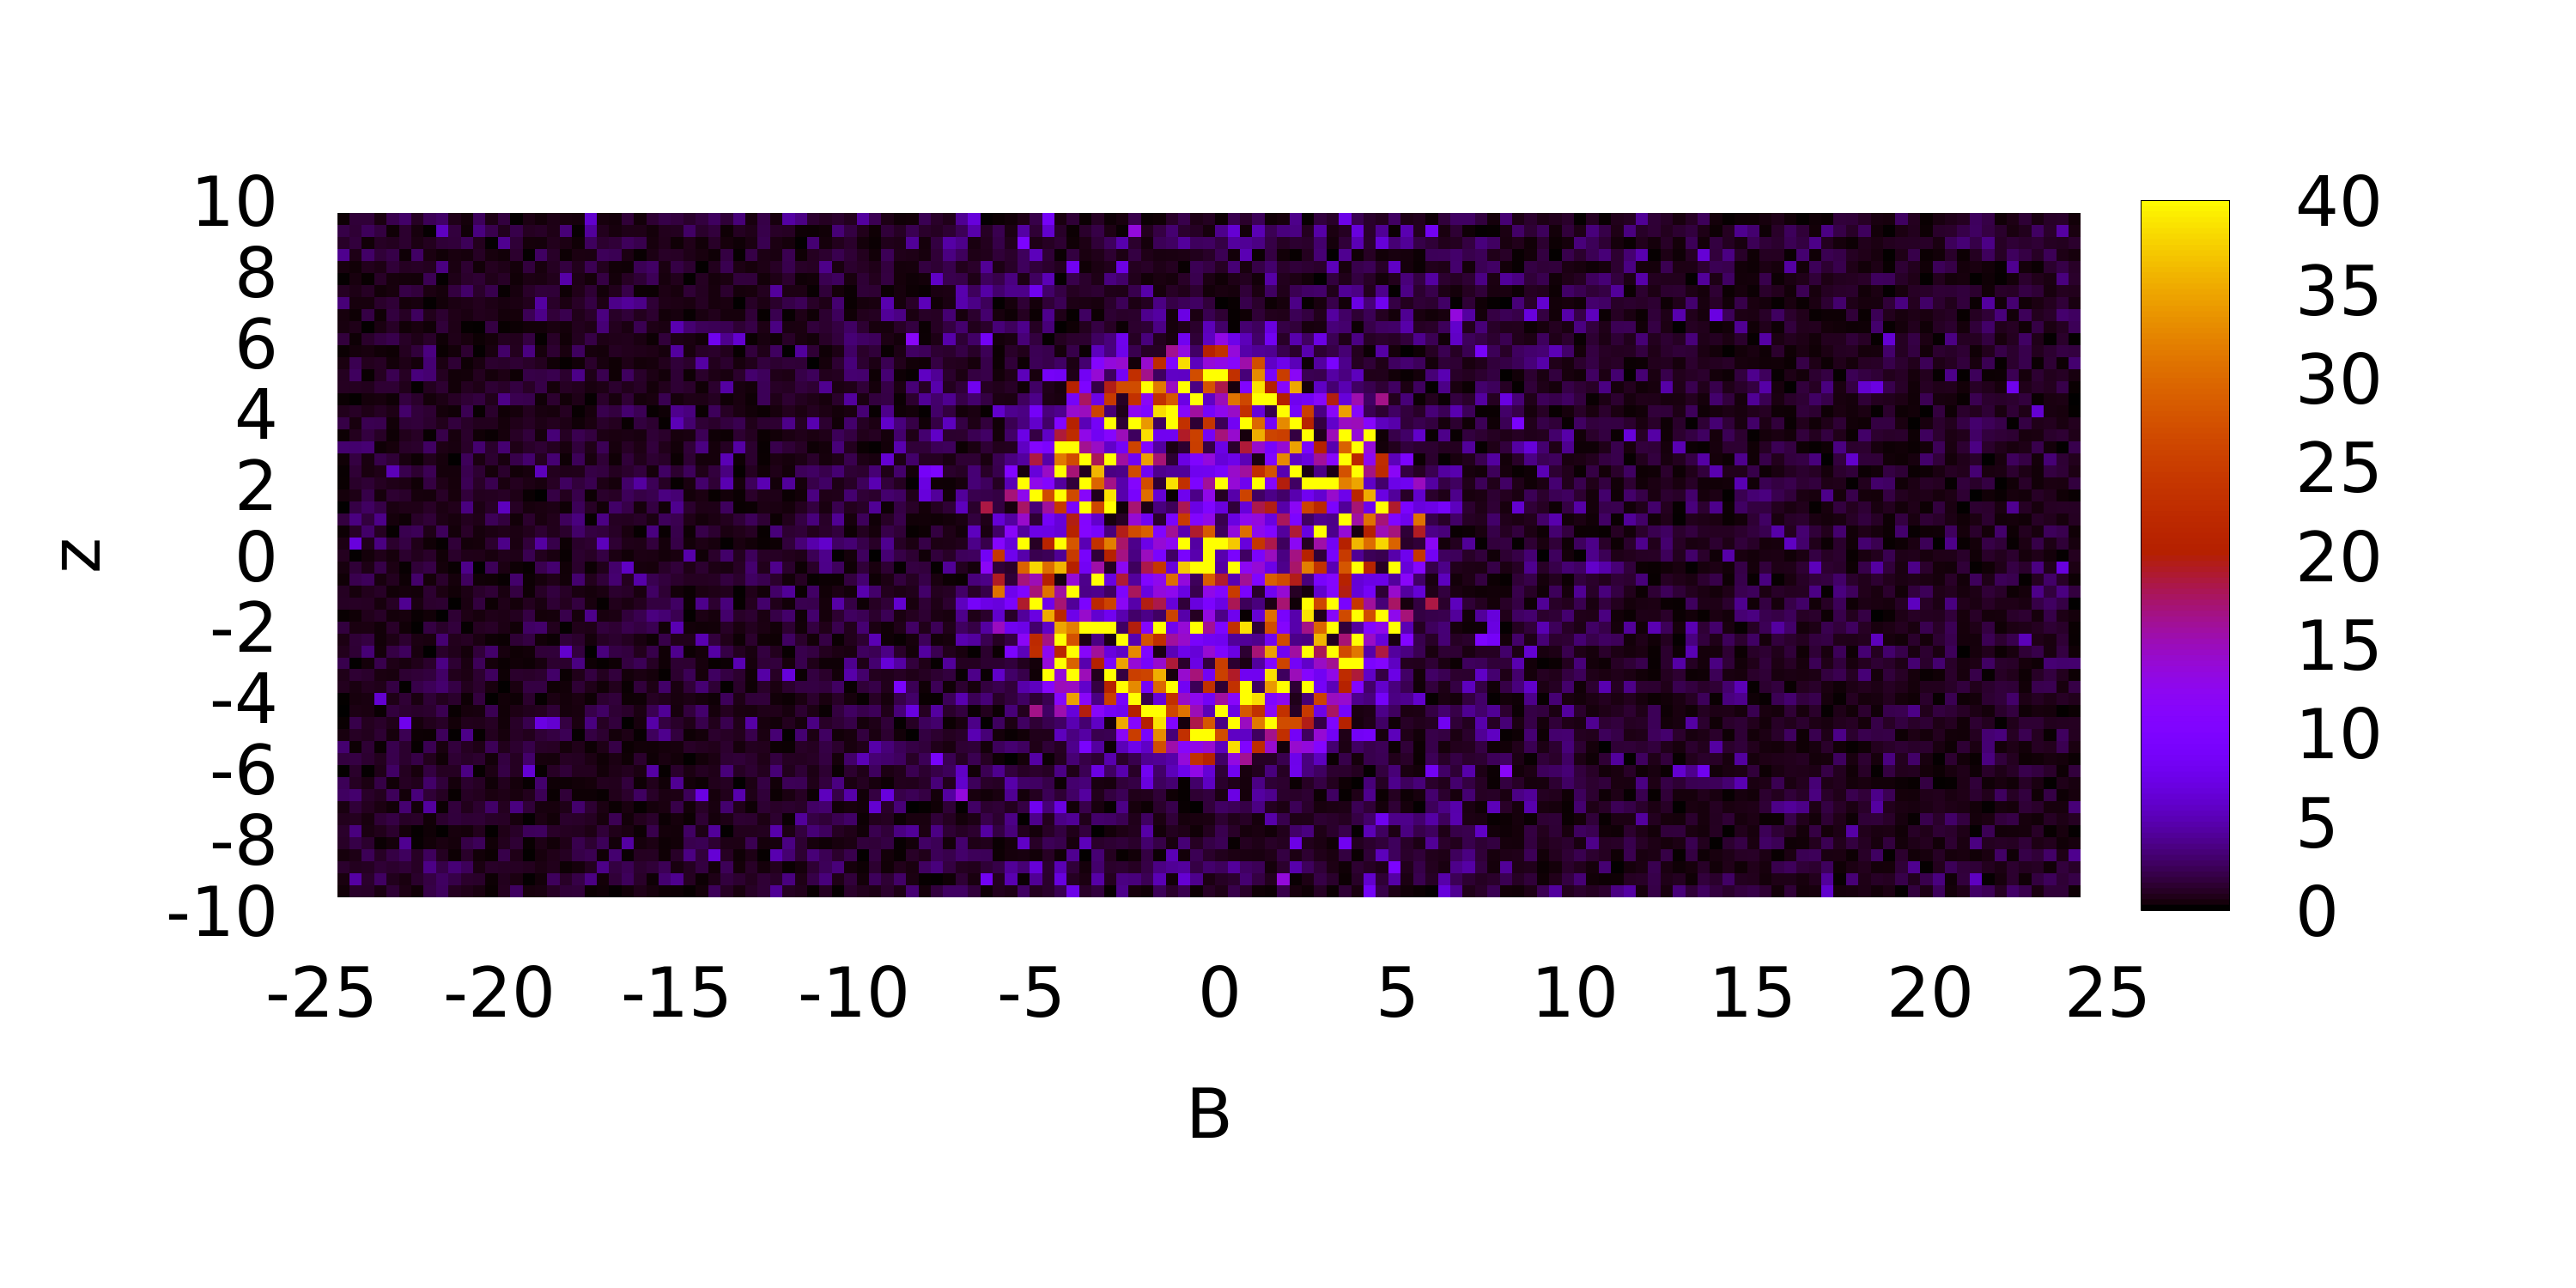
\includegraphics[width=0.7\columnwidth]{Syz_noB.png}
    \caption{Structure factor $S(0, q_y, q_z)$ of the system in absence of magnetic field.}
    \label{fig:Syz_noB}
\end{figure}


\subsection{Pair distribution function}

Likewise the case with a magnetic field, it has been calculated the pair distribution function of a system of spherocylinders in absence of magnetic field. As it can be seen from Fig. \ref{fig:gxz_noB} and Fig. \ref{fig:gyz_noB}, the phase is clearly isotropic, without long range spatial correlation between the particles, corroborating the magnetic field induced nature of the smectic phase.


\begin{figure}
    \centering
    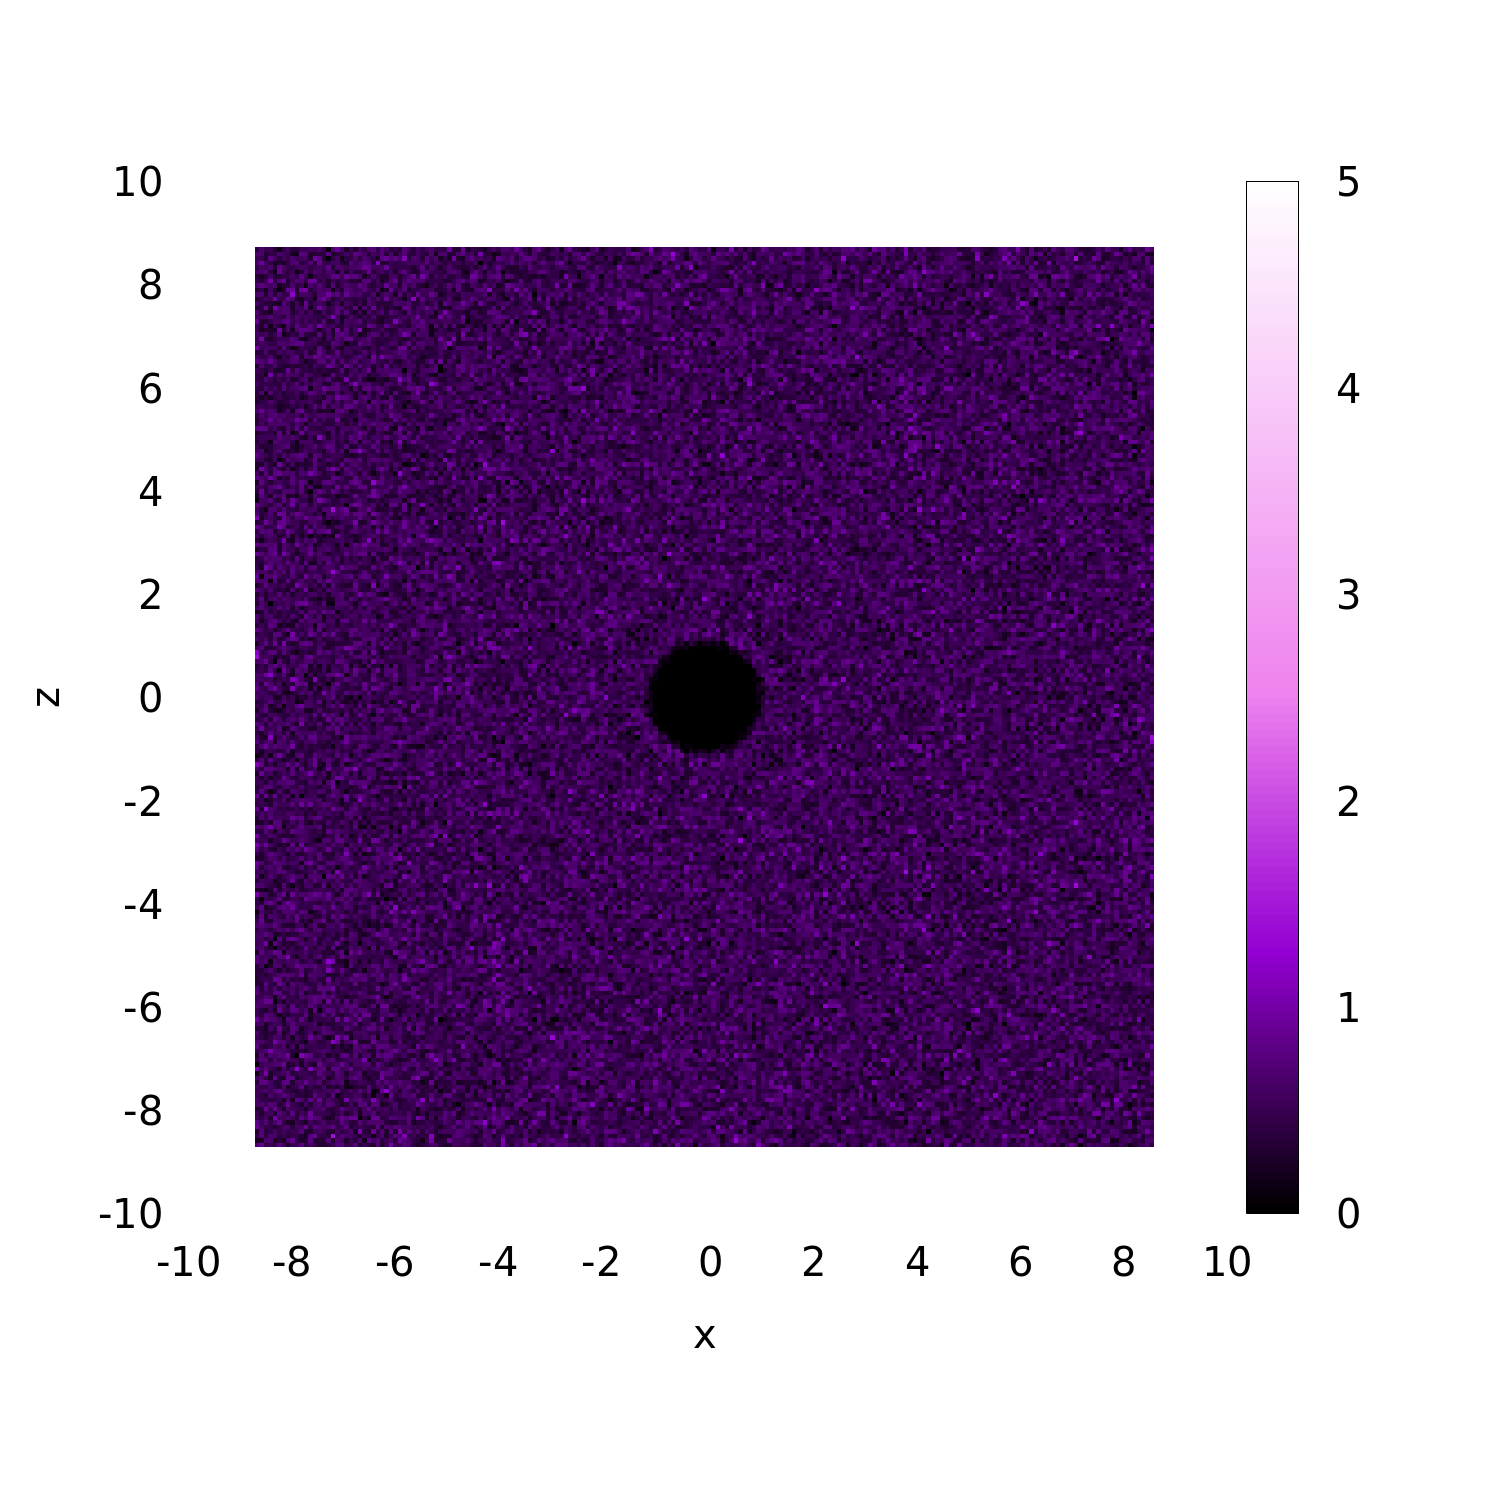
\includegraphics[width=0.7\columnwidth]{gxz_noB.png}
    \caption{Pair distribution function of the system on the xz-plane without a magnetic field.}
    \label{fig:gxz_noB}
\end{figure}

fix
\begin{figure}
    \centering
    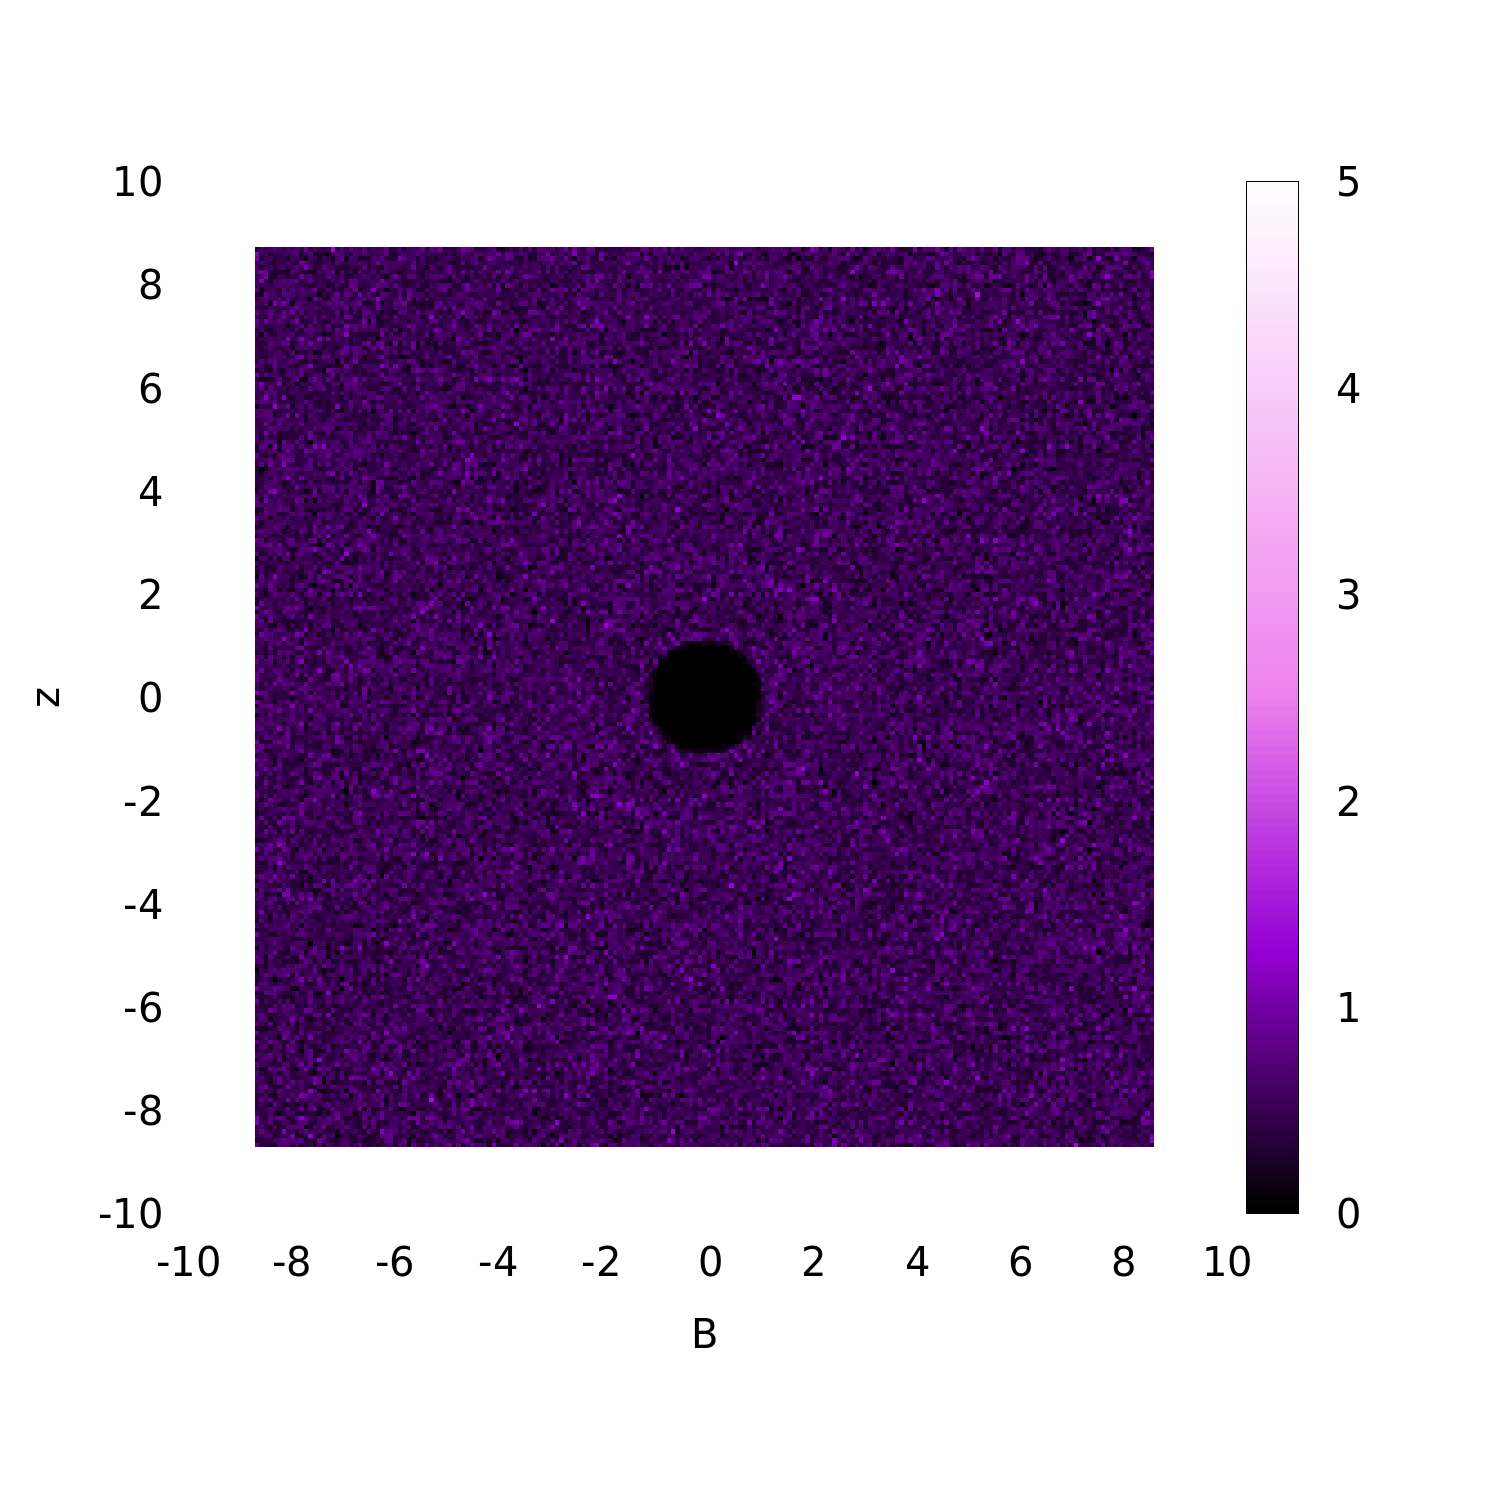
\includegraphics[width=0.7\columnwidth]{gyz_noB.png}
    \caption{Pair distribution function of the system on the yz-plane without a magnetic field.}
    \label{fig:gyz_noB}
\end{figure}

\newpage

\section{Smectic and nematic ordering}

A convenient way to check for the emergence of a smectic phase in our computer simulations 
is to calculate the smectic order parameter $\tau_1$ defined as follows:

\begin{equation}
    \tau_1 = \langle | \sum_i e^{i 2\pi \vec{r}_i \cdot \hat{n} / d } |\rangle 
\end{equation}

where $\langle\ldots\rangle$ is an average over several independent configurations, $\vec{r}_i$ is the position of the $i$-th particle, $\hat{n}$ is the direction of the magnetic
field and $d$ is the thickness of the smectic layers.
In order to compute $\tau_1$ for each configuration we find the optimal value of $d$, i.e. 
the value which maximizes $\tau_1$.

The values of $\tau_1$ for both HSCs and HEs and for all pressures studied is shown in Fig.~\ref{fig:ordpars}(top). It can be seen that HSCs exhibit a range of volume fractions where 
a smectic layer ordering is present and which coincide with the green state points shown in Fig. 7(a)
in the main test. On the contrary no evidence of layering emerges in the simulation of HEs.

\begin{figure}
    \centering
    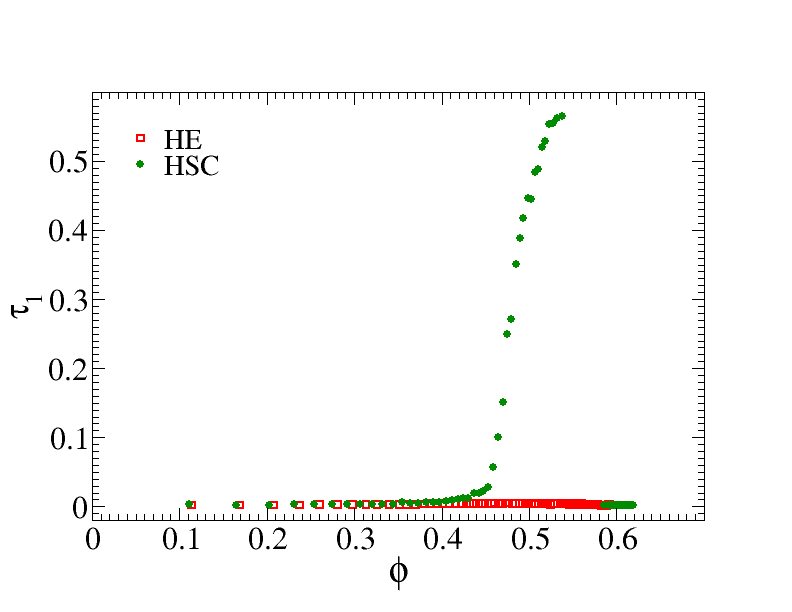
\includegraphics[width=0.7\columnwidth]{smordpar.png}
    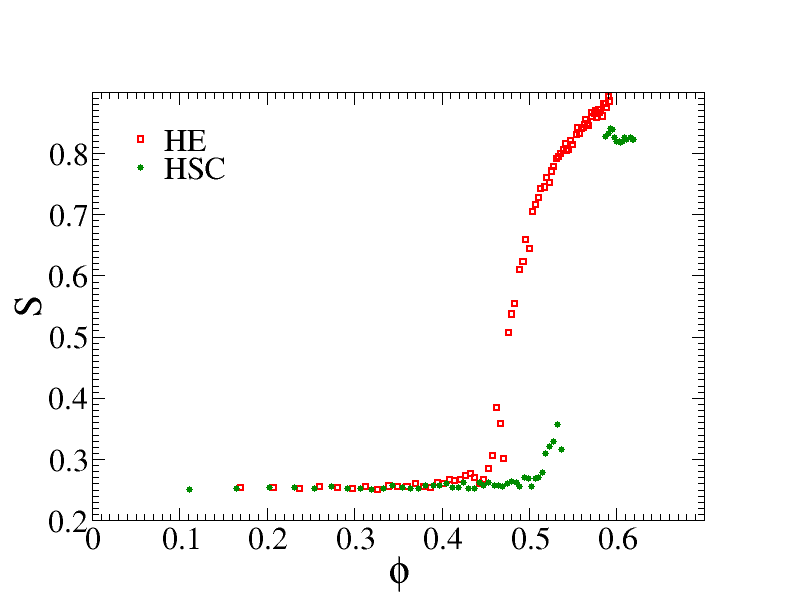
\includegraphics[width=0.7\columnwidth]{nemop.png}  
    \caption{Smectic ($\tau_1$, top) and nematic ($S$, bottom) order parameters for HSCs and HEs.}
    \label{fig:ordpars}
\end{figure}

We also calculated the nematic order parameter $S$ related to the symmetry axis of HSC and HE, which
is defined as the largest eigenvalue of the order tensor $Q$, whose components are:
\begin{equation}
Q_{\alpha\beta} = \frac{1}{N} \sum_i \frac{3}{2} \langle (\mathbf{u}_i)_\alpha (\mathbf{u}_i)_\beta\rangle
\label{eq:nemop}
\end{equation}
where $\alpha\beta\in\{x,y,z\}$ and the unit vector $(\mathbf{u}_i)_\alpha$ is the component $\alpha$ of the orientation (i.e. the symmetry axis) of particle $i$.
First we note that since particles are aligned perpendicularly to the nematic field, if they are 
randomly oriented one has $S=1/4$. Hence, below $\phi_0 < 0.45$ both symmetry axis of HSC and HE are 
randomly oriented onto the plance perpendicular to the magnetic field.
Interestingly, for $\phi > \phi_0$ HSC starts exhibiting smectic layering but their orientations
remain random, while orientations of HE starts aligning (see Fig.~\ref{fig:ordpars}(bottom)).

\section{Shape analysis}

The particular behaviour of the particles can be understood by analysing their shape. In particular, it has been obtained the particle borders from a pool of samples belonging to the two aspect ratios ($\rho_1 = 2.82, \rho_2 = 3.69$). By developing a C++ program, the coordinates of the borders have been analysed and fitted using an ellipse and a spherocylinder shape. Due to the anisotropy of the particles, the analisys has been performed on the left and on the right side of the particles independently (Fig. \ref{fig:Part_fit}). The fit minimizes the distance $d$ between the border coordinates of a particle and the nearest point of the fitting shape. The hybrid nature of the particles is easy to notice, particularly using a spherocylindrical fit which is very sensible to the flatness of the particle sides. The results of this analysis are represented in the histograms in Fig. \ref{fig:Mean_dist}. As it can be easily noticed, the analysis on the more elongated particles ($\rho = 3.69$) shows their almost ellipsoidal nature, leading to a lower mean distance. On the contrary, the particles with $\rho = 2.82$ present a more hybrid nature, with a comparable mean distance distribution between the two fits.

\begin{figure}
    \centering
    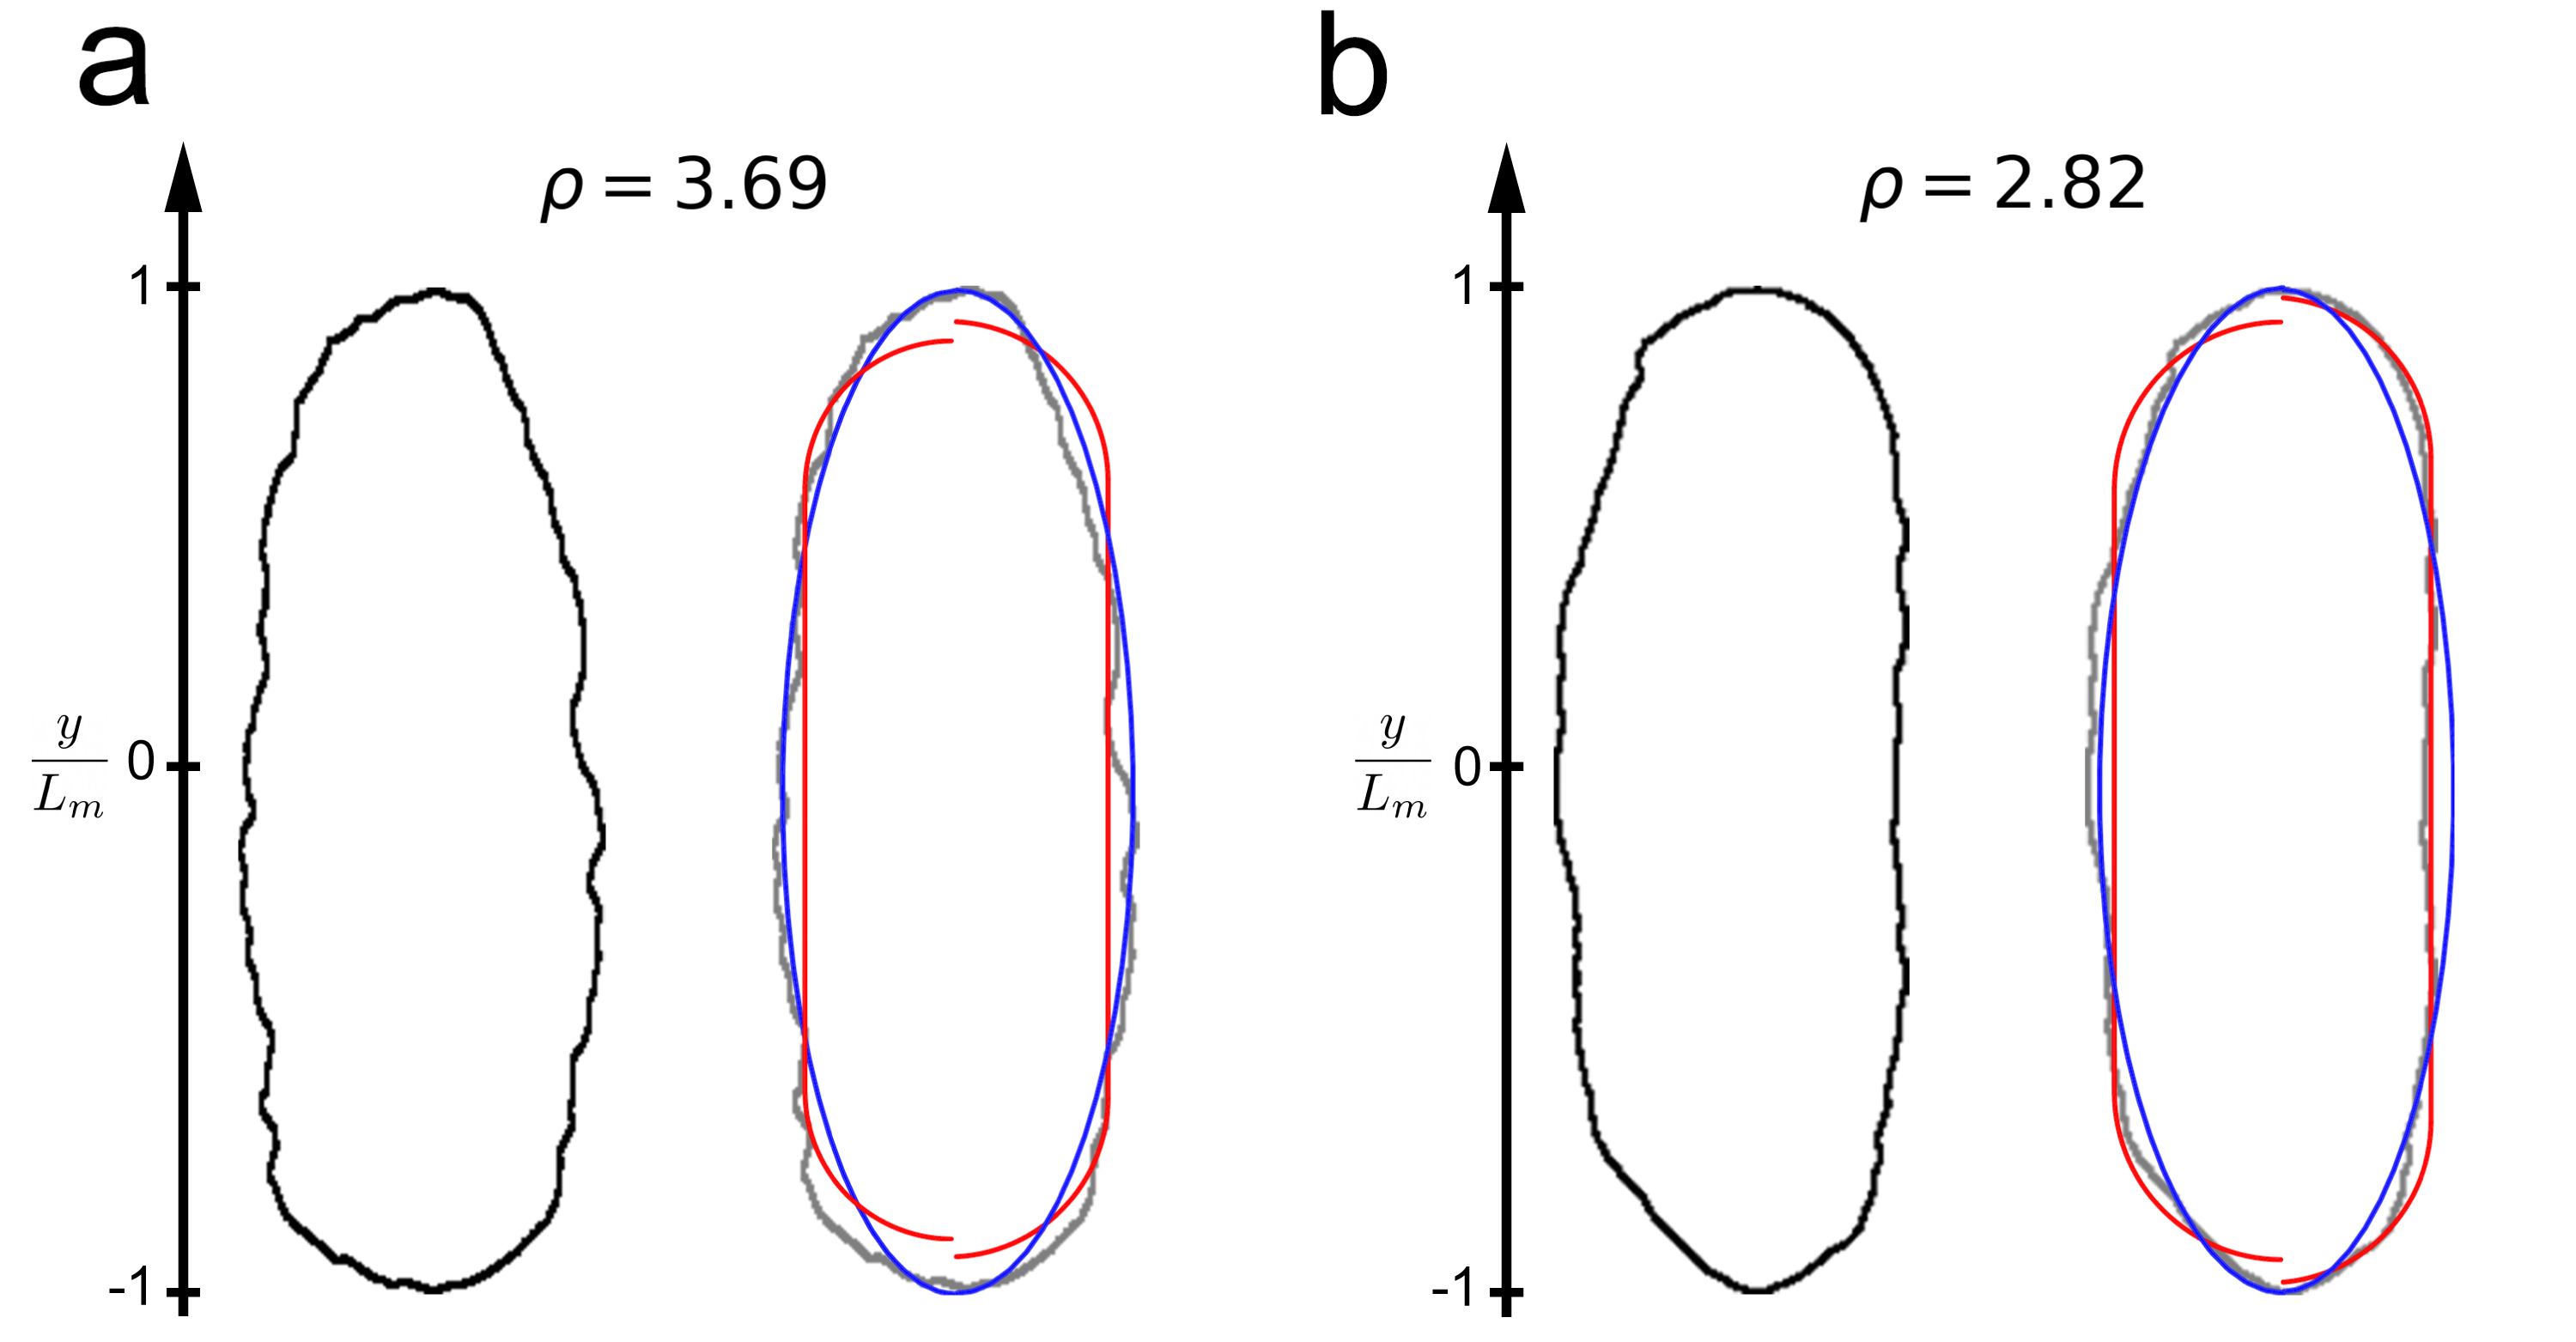
\includegraphics[width=0.7\columnwidth]{Part fit.png}
    \caption{Particle shape analysis. The border of the particles with $\rho = 3.69$ (a) and $\rho = 2.82$ (b) has been fitted using an ellipse (in blue) and a spherocylinder (in red).}
    \label{fig:Part_fit}
\end{figure}


\begin{figure}
    \centering
    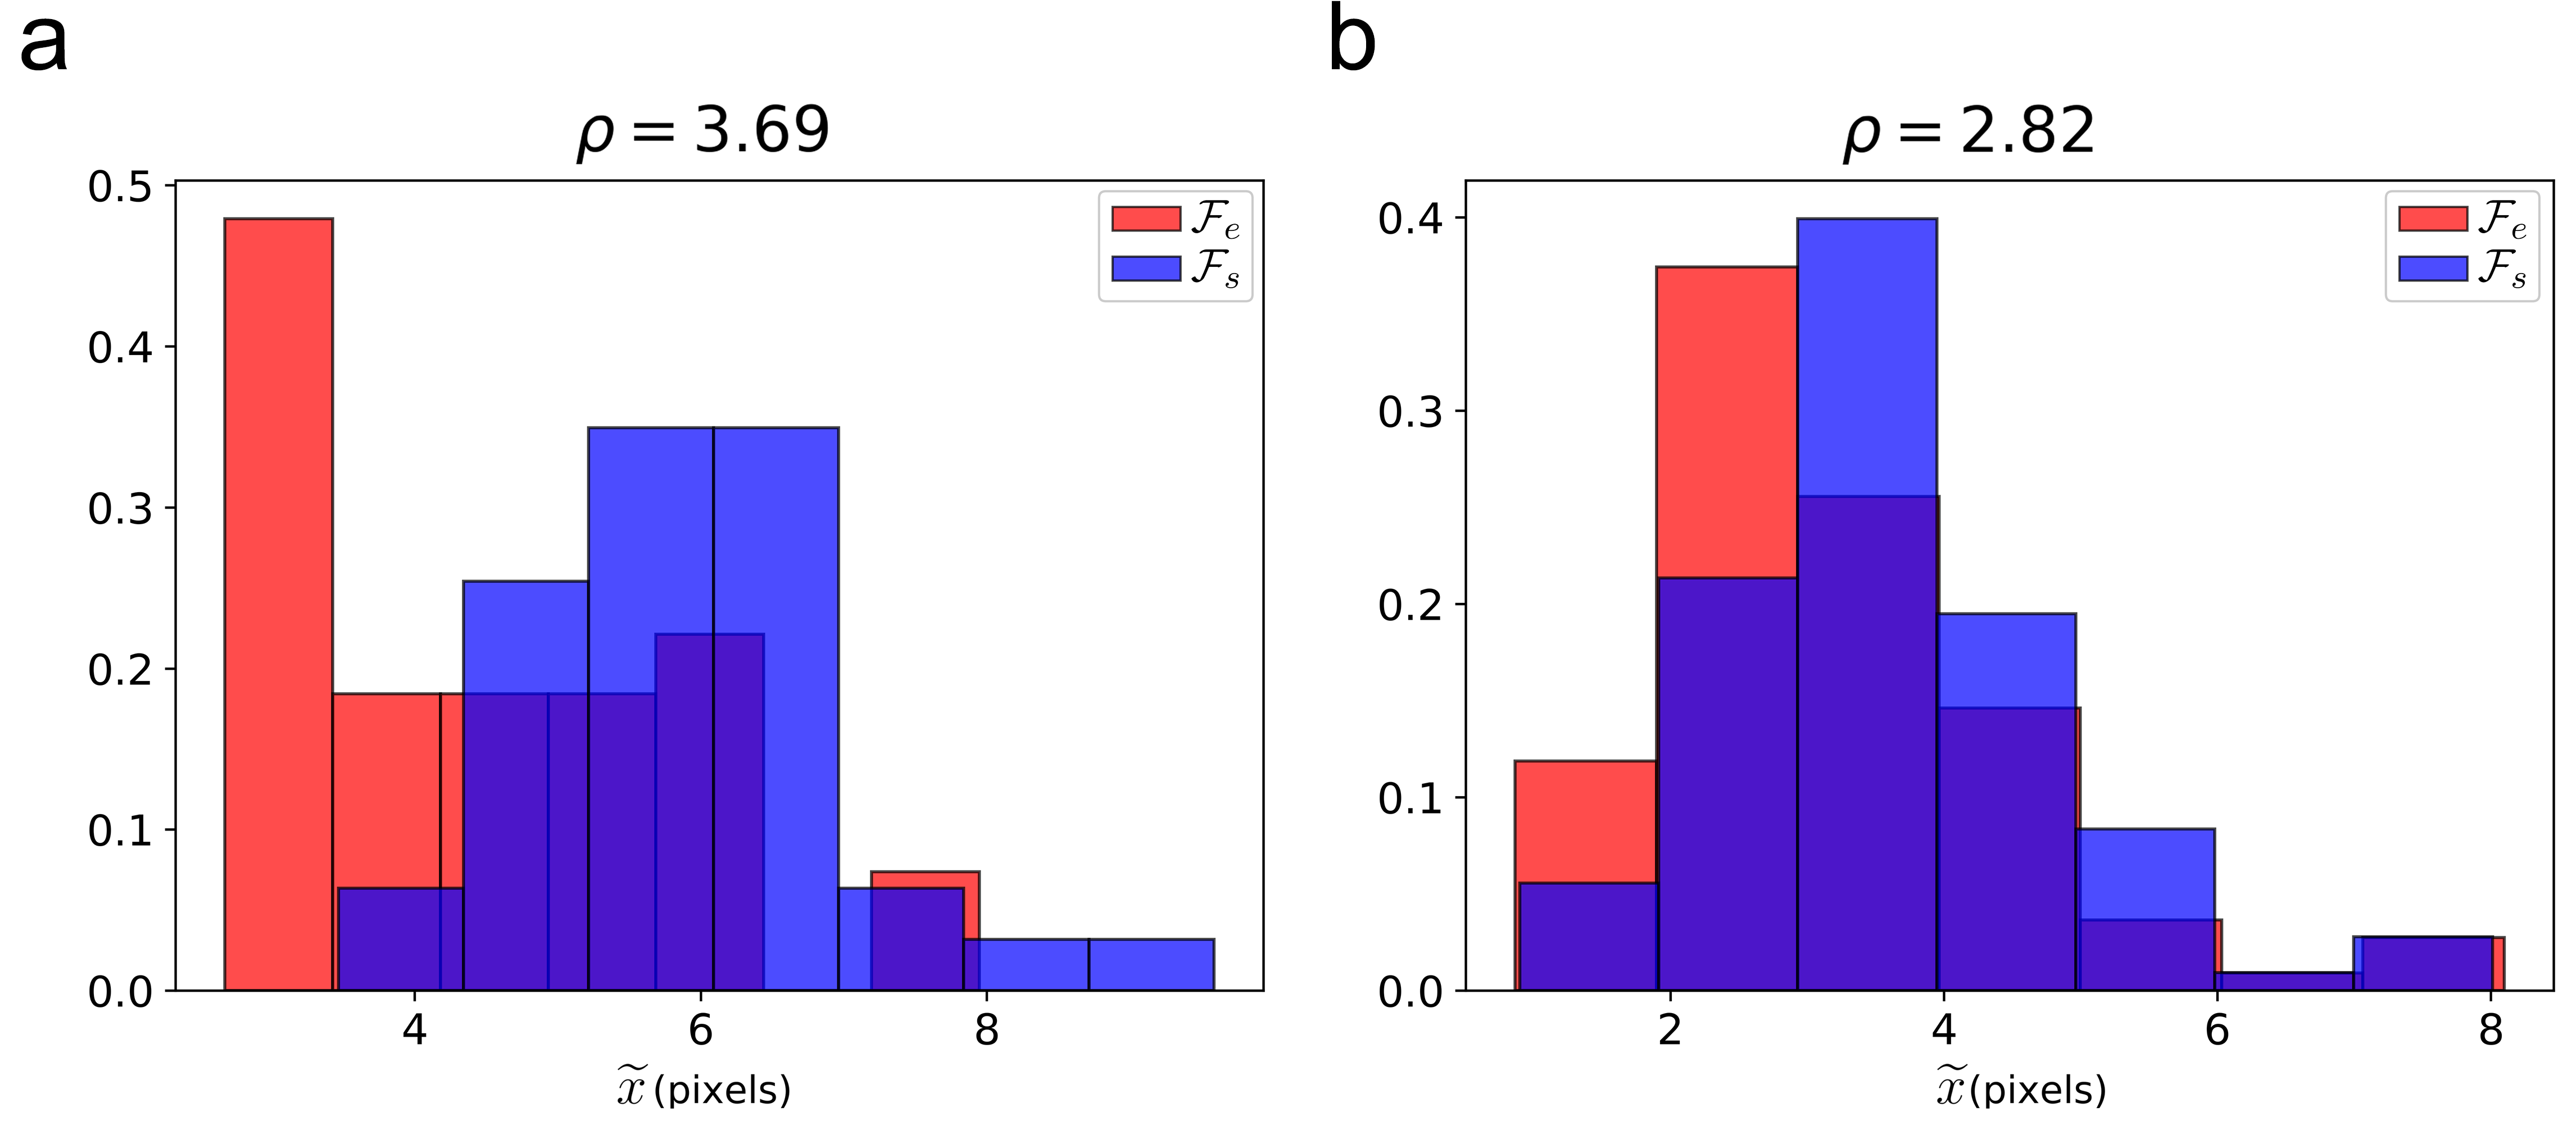
\includegraphics[width=0.7\columnwidth]{Mean_dist.png}
    \caption{Probability density of the minimum mean distance $d$ between the border of the particles ($\rho = 3.69$ (a) and $\rho = 2.82$ (b)) and the fitting shape.}
    \label{fig:Mean_dist}
\end{figure}

In order to analyse further the shape of the particles, the border of the two pools have been averaged and fitted as before, leading to Fig. \ref{fig:Mean_bord}a. In Fig. \ref{fig:Mean_bord}b is represented the mean squared distance $d^2$ of the fit as a function of the normalised position in respect to the centre of the particle. As it can be observed, the ellispoidal fit raises its $d^2$ moving from $\rho=3.69$ to $\rho=2.82$ while the spherocylindrical one becomes lower, remarking again the more hybrid nature of the particles with $\rho=2.82$.

\begin{figure}
    \centering
    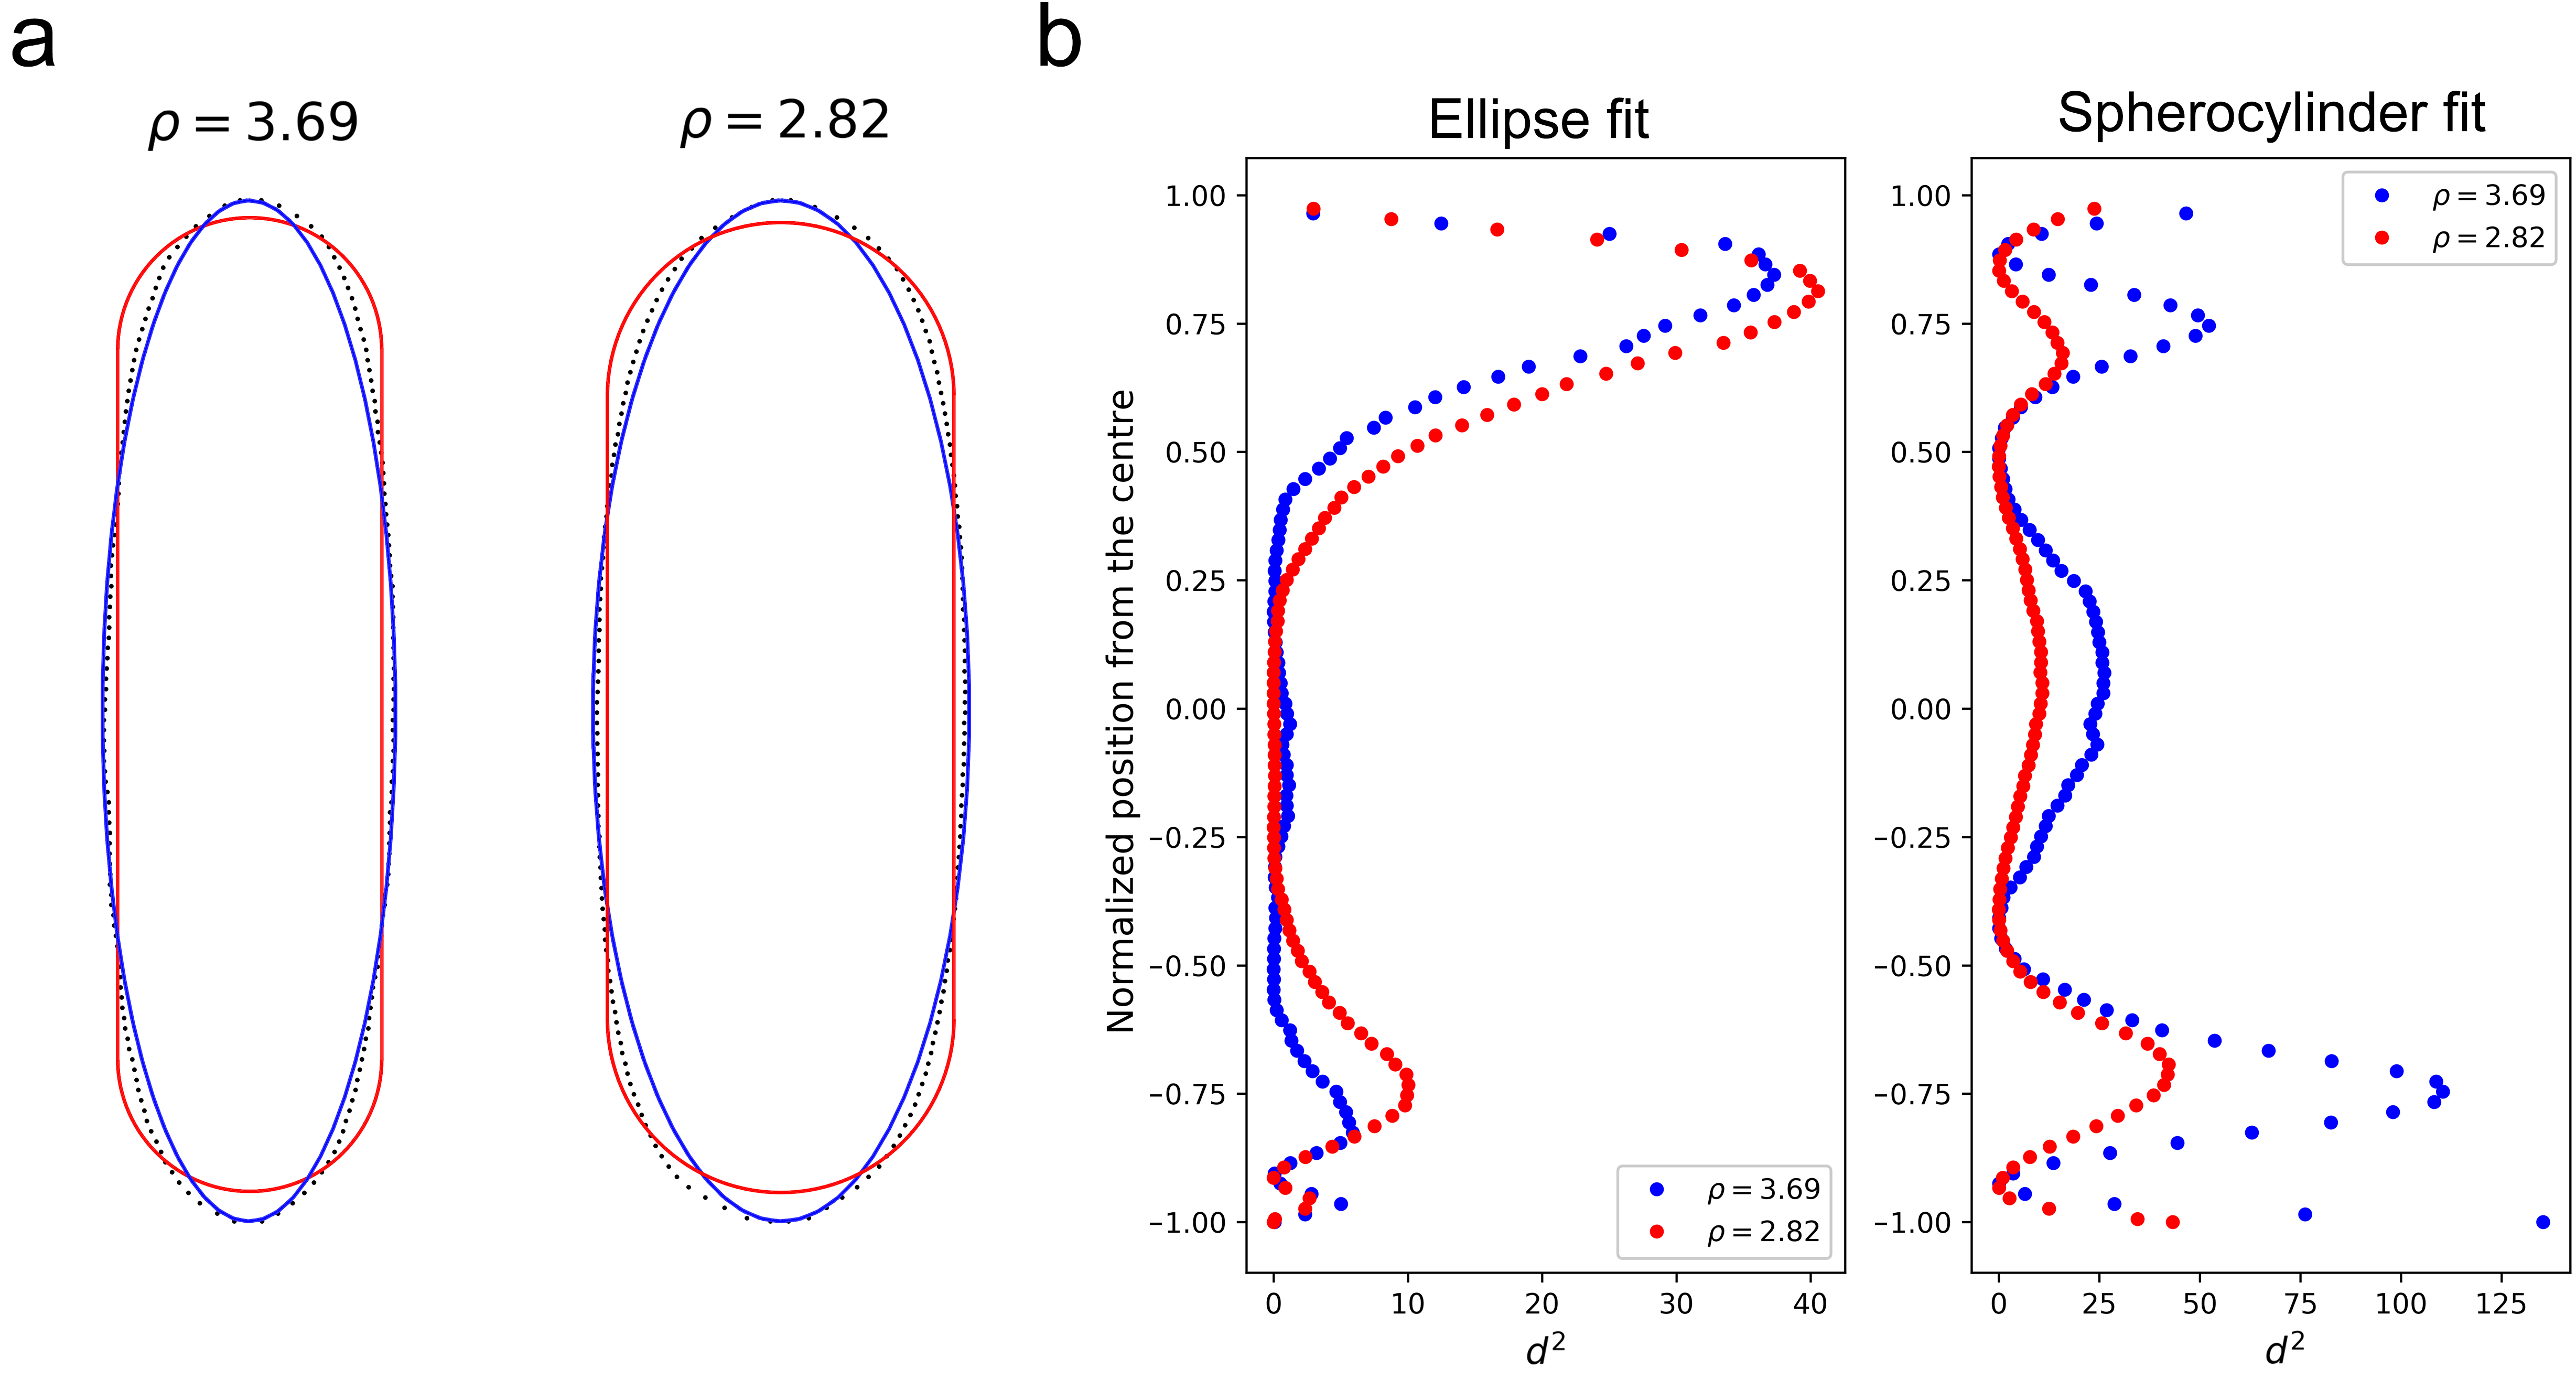
\includegraphics[width=0.7\columnwidth]{Mean_bord.png}
    \caption{(a) Average border of the particles with the two $\rho$ (black dots). Superposed are represented the two different fits that have been performed (ellipse in blue and spherocylinder in red). (b) Mean squared distance of the border from the fits as a function of the normalised distance from the centre, which corresponds to the $0$ of the vertical axis.}
    \label{fig:Mean_bord}
\end{figure}

Thus, the particles can't be described as ellipses neither spherocylinders, instead as a intermediate shape. Hence, to demonstrate the different behaviour of these two types of particles it has been calculated the flatness of the particles as follows. Starting from the middle section of the particles, it has been performed a linear fit of the border, calculating the mean distance $d$ of the border from the fitting line. Then, repeating the procedure while adding more fitting points, we calculated the maximum distance from the centre of the particle which presented a mean distance $d$ less than a threshold, i. e. $d < 5$. The result of this analysis, represented int Fig. \ref{fig:maxlength_div}, shows that the particles with $\rho=2.82$ presents a much longer flat portion in respect to those with $\rho=3.69$. This flatness can be the reason why the particles with $\rho=2.82$, even though not being perfect spherocylinders, resembles more their behaviour, while keeping the N transition typical of ellipsoids. 

\begin{figure}
    \centering
    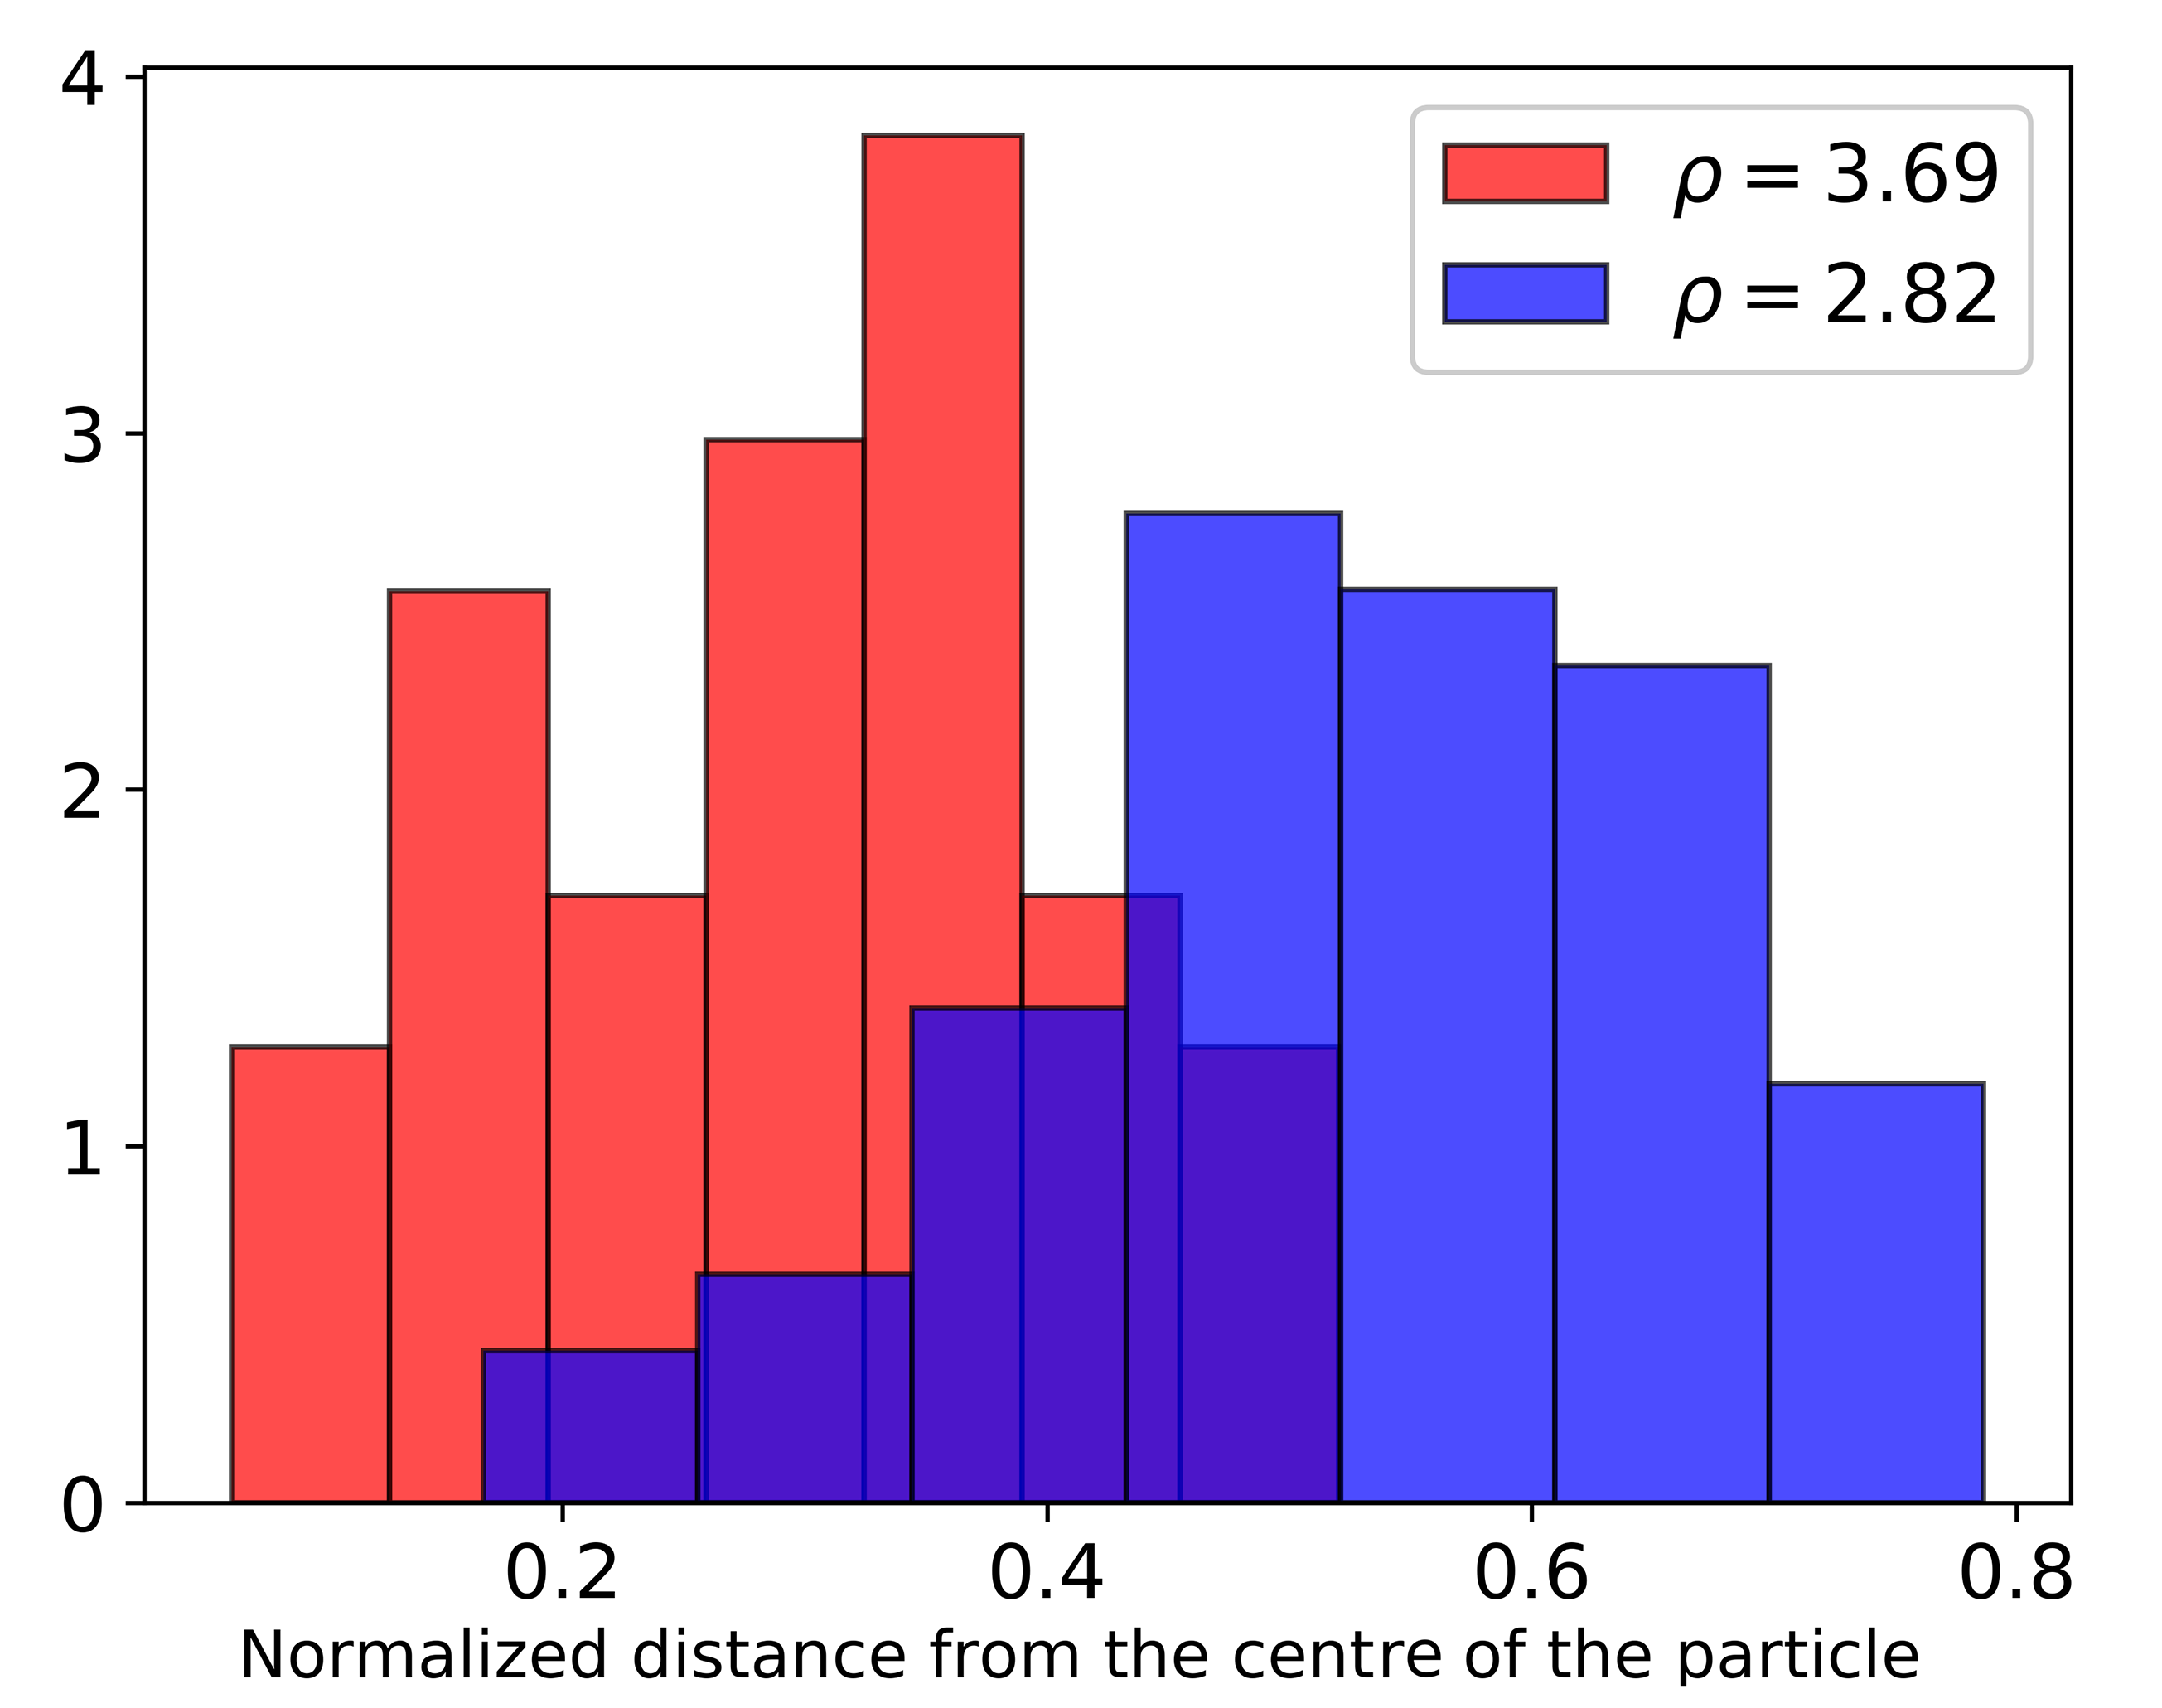
\includegraphics[width=0.7\columnwidth]{maxlength_div.png}
    \caption{Probability density of the flat portion of the particles with the two different aspect ratios: $\rho=3.69$ in red and $\rho=2.82$ in blue.}
    \label{fig:maxlength_div}
\end{figure}

\bibliography{ref_dubble}


\end{document}
